\documentclass[11pt,a4paper]{article}
%%%----------------------------------------------------------------------------%%%
%%%----------------------------------------------------------------------------%%%
%%% 
%%% ### Packages 
%%%
%%%----------------------------------------------------------------------------%%%
%%%----------------------------------------------------------------------------%%%
\usepackage{amsmath, amsthm, amssymb, nccbbb, bm, dsfont, pifont, fontawesome, graphicx, varioref, enumitem, mathtools, listings, xcolor, cite}
\RequirePackage[round,authoryear]{natbib}
\RequirePackage[colorlinks,citecolor=blue,urlcolor=blue]{hyperref}
\usepackage[cal=boondox]{mathalfa}
%\usepackage[numbers]{natbib}
\setlength{\topmargin}{-1in}
\setlength{\textheight}{10.5in}
\setlength{\oddsidemargin}{-.6in}
\setlength{\textwidth}{7.5in}
\hypersetup{colorlinks=true, linkcolor=blue, citecolor=red, urlcolor=blue}

%%%----------------------------------------------------------------------------%%%
%%%----------------------------------------------------------------------------%%%
%%% 
%%% ### Code 
%%%
%%%----------------------------------------------------------------------------%%%
%%%----------------------------------------------------------------------------%%%
\usepackage{listings}
\lstset{escapeinside=| |}
\usepackage[usenames,dvipsnames]{color}  
\definecolor{mygray}{rgb}{0.99,0.99,0.99}
\definecolor{myblue}{rgb}{0.0, 0.23, 0.63}
\definecolor{myred}{rgb}{0.75, 0.0, 0.0}
\definecolor{mygreen}{rgb}{0.4, 0.69, 0.2}  
\lstnewenvironment{R}{\lstset{ 
  language=R,
  basicstyle=\footnotesize\ttfamily, 
  numbers=left,
  numberstyle=\tiny\color{black},
  stepnumber=1,
  numbersep=5pt,
  backgroundcolor=\color{mygray},
  showspaces=false, 
  showstringspaces=false,
  showtabs=false, 
  frame=single,  
  rulecolor=\color{black},
  tabsize=4,
  captionpos=b,
  breaklines=true,
  breakatwhitespace=false,
  keywordstyle=\ttfamily\bfseries\color{myblue},
  commentstyle=\ttfamily\bfseries\color{myred},
  stringstyle=\ttfamily\bfseries\color{mygreen}
} 
}{}

%New colors defined below
\definecolor{codegreen}{rgb}{0,0.6,0}
\definecolor{codegray}{rgb}{0.5,0.5,0.5}
\definecolor{codepurple}{rgb}{0.58,0,0.82}
\definecolor{backcolour}{rgb}{0.95,0.95,0.92}

%Code listing style named "mystyle"
\lstdefinestyle{mystyle}{
  backgroundcolor=\color{backcolour}, commentstyle=\color{codegreen},
  keywordstyle=\color{magenta},
  numberstyle=\tiny\color{codegray},
  stringstyle=\color{codepurple},
  basicstyle=\ttfamily\footnotesize,
  breakatwhitespace=false,         
  breaklines=true,                 
  captionpos=b,                    
  keepspaces=true,                 
  numbers=left,                    
  numbersep=5pt,                  
  showspaces=false,                
  showstringspaces=false,
  showtabs=false,                  
  tabsize=2
}

%"mystyle" code listing set
\lstset{style=mystyle}

%%%----------------------------------------------------------------------------%%%
%%%----------------------------------------------------------------------------%%%
%%% 
%%% ### Box
%%%
%%%----------------------------------------------------------------------------%%%
%%%----------------------------------------------------------------------------%%%
\usepackage{tcolorbox}
\tcbuselibrary{breakable}
\newtcolorbox{mybox}{colback=yellow!5!white, colframe=gray!60!black, breakable}
\newtcolorbox{mybox0}{colback=white, colframe=gray!60!black, breakable}
	

%%%----------------------------------------------------------------------------%%%
%%%----------------------------------------------------------------------------%%%
%%% 
%%% ### Theorem style structures 
%%%
%%%----------------------------------------------------------------------------%%%
%%%----------------------------------------------------------------------------%%%
\numberwithin{equation}{section}
\theoremstyle{plain}
\newtheorem{theorem}{Theorem}[section]
\newtheorem{lemma}[theorem]{Lemma}
\newtheorem{corollary}[theorem]{Corollary}
\newtheorem{proposition}[theorem]{Proposition}
\newtheorem{condition}{Condition}[section]
\newtheorem{definition}{Definition}[section]
\theoremstyle{definition}
\newtheorem{example}{Example}[section]
\newtheorem{exercise}{Exercise}[section]
\newtheorem{remark}{Remark}[section]
\newtheorem{remark0}{Remark}
\newtheorem{question}{Question}


%%%----------------------------------------------------------------------------%%%
%%%----------------------------------------------------------------------------%%%
%%% 
%%% ### Operators 
%%%
%%%----------------------------------------------------------------------------%%%
%%%----------------------------------------------------------------------------%%%
\newcommand{\pr}{\mathsf{P}} 
\newcommand{\E}{\mathsf{E}} 
\newcommand{\median}{\mathop{\mathsf{median}}}
\newcommand{\Cov}{{\mathsf{Cov}}} 
\newcommand{\Corr}{{\mathsf{Corr}}} 
\newcommand{\Var}{{\mathsf{Var}}}
\newcommand{\SD}{{\mathsf{SD}}}
\newcommand{\CV}{{\mathsf{CV}}}
\newcommand{\Bias}{{\mathsf{Bias}}}
\newcommand{\AMSE}{\operatorname{\mathsf{AMSE}}}
\newcommand{\MSE}{\operatorname{\mathsf{MSE}}}
\newcommand{\ARE}{\mathsf{ARE}}
\newcommand{\AV}{\mathsf{AV}}
\newcommand{\CRLB}{{\mathsf{CRLB}}}

\newcommand{\pCorr}{\text{P}}
\newcommand{\sCorr}{\text{S}}
\newcommand{\kCorr}{\text{K}}
\newcommand{\bdCorr}{\text{BD}}
\newcommand{\cCorr}{\text{C}}


\newcommand{\inD}{    \overset{ \textnormal{d}   }{\rightarrow} }
\newcommand{\inAS}{   \overset{ \textnormal{a.s.}   }{\rightarrow} }
\newcommand{\inP}{    \overset{ \textnormal{pr}    }{\rightarrow} }
\newcommand{\inLp}{   \overset{ \mathcal{L}^p }{\rightarrow} }
\newcommand{\inMSE}{  \overset{ \textnormal{qm} }{\rightarrow} }
\newcommand{\inQM}{   \overset{ \textnormal{qm} }{\rightarrow} }
\newcommand{\indep}{\protect\mathpalette{\protect\independenT}{\perp}}
\def\independenT#1#2{\mathrel{\rlap{$#1#2$}\mkern4mu{#1#2}}}
\newcommand{\iid}{\textsc{iid}} 
\newcommand{\simIID}{   \overset{ \iid   }{\sim} }
\newcommand{\simIND}{   \overset{ {\indep}   }{\sim} }


\newcommand{\Bern}{\textnormal{Bern}} 
\newcommand{\Unif}{\textnormal{Unif}} 
\newcommand{\Normal}{\textnormal{N}} 
\newcommand{\logNormal}{\textnormal{LN}} 
\newcommand{\Bin}{\textnormal{Bin}} 
\newcommand{\NB}{\textnormal{NB}} 
\newcommand{\HG}{\textnormal{HG}} 
\newcommand{\Geom}{\textnormal{Geom}} 
\newcommand{\Beta }{\textnormal{Beta}} 
\newcommand{\BetaBin}{\textnormal{Beta-Bin}}
\newcommand{\Ga}{\textnormal{Ga}} 
\newcommand{\Exp}{\textnormal{Exp}} 
\newcommand{\Expo}{\textnormal{Expo}} 
\newcommand{\Po}{\textnormal{Po}} 
\newcommand{\Multi}{\textnormal{Multi}} 
\newcommand{\student}{\textnormal{t}} 
\newcommand{\Cauchy}{\textnormal{Cauchy}} 
\newcommand{\Pareto}{\textnormal{Pareto}} 
\newcommand{\Laplace}{\textnormal{Laplace}} 
\newcommand{\Logistic}{\textnormal{Logistic}} 
\newcommand{\Dir}{\textnormal{Dir}} 
\newcommand{\DP}{\textnormal{DP}} 
\newcommand{\Inv}{\textnormal{Inv-}} 
\newcommand{\F}{\textnormal{F}} 
\newcommand{\sign}{\textnormal{sign}}
\newcommand{\rank}{\textnormal{rank}}


\newcommand{\RV}{\textsc{rv}}
\newcommand{\cdf}{\textsc{cdf}} 
\newcommand{\cgf}{\textsc{cgf}} 
\newcommand{\pdf}{\textsc{pdf}} 
\newcommand{\pmf}{\textsc{pmf}} 
\newcommand{\chf}{\textsc{chf}} 
\newcommand{\mgf}{\textsc{mgf}}
\newcommand{\EF}{\textsc{EF}}
\newcommand{\NEF}{\textsc{NEF}}
\newcommand{\MLE}{\textsc{mle}}
\newcommand{\MAP}{\textsc{MAP}}
\newcommand{\Med}{\textsc{Med}}
\newcommand{\MME}{\textsc{mme}}
\newcommand{\QME}{\textsc{qme}}
\newcommand{\UMVUE}{\textsc{umvue}}
\newcommand{\MPT}{\textsc{MPT}}
\newcommand{\UMPT}{\textsc{UMPT}}
\newcommand{\LRT}{\textsc{LRT}}


\newcommand{\diag}{\mathop{\mathrm{diag}}}
\newcommand{\tr}{\mathop{\mathrm{tr}}}
\newcommand{\T}{\mathop{\mathrm{T}}}
\DeclareMathOperator*{\argmin}{arg\,min}
\DeclareMathOperator*{\argmax}{arg\,max}
\DeclareMathOperator{\sgn}{sgn}
\DeclareMathOperator{\logit}{logit}
\DeclareMathOperator{\expit}{expit}
\newcommand{\dd}{\textnormal{d}}


\newcommand{\lva}{{\color{myred}\ding{73}\ding{73}\ding{73}}}
\newcommand{\lvb}{{\color{myred}\ding{72}\ding{73}\ding{73}}}
\newcommand{\lvc}{{\color{myred}\ding{72}\ding{72}\ding{73}}}
\newcommand{\lvd}{{\color{myred}\ding{72}\ding{72}\ding{72}}}
\newcommand{\optional}{\noindent{\color{myblue}\faScissors}}
\newcommand{\Solution}{\noindent{\color{myblue}{{\textsc{Solution}}:~$\Big.$}}}
\newcommand{\take}{\noindent{\color{myblue}\faPaperPlaneO~\underline{\bf Takeaway}:~$\Big.$}}

% widecheck 
\DeclareFontFamily{U}{mathx}{\hyphenchar\font45}
\DeclareFontShape{U}{mathx}{m}{n}{
      <5> <6> <7> <8> <9> <10>
      <10.95> <12> <14.4> <17.28> <20.74> <24.88>
      mathx10
      }{}
\DeclareSymbolFont{mathx}{U}{mathx}{m}{n}
\DeclareFontSubstitution{U}{mathx}{m}{n}
\DeclareMathAccent{\widecheck}{0}{mathx}{"71}
\DeclareMathAccent{\wideparen}{0}{mathx}{"75}

\def\cs#1{\texttt{\char`\\#1}}

\newcounter{magicrownumbers}
\newcommand\rownumber{\stepcounter{magicrownumbers}\arabic{magicrownumbers}}

\usepackage[table]{xcolor}
%------------------------------------------------------------------------------



\begin{document}
    % Page 0 for names and table of contents
    \thispagestyle{empty}
    \pagenumbering{gobble} 
    \title{\textsc{RMSC 4002} -- Financial Data Analytics with Machine Learning \\ Group Project}
    \author{
        CHOI Sen Hei (SID: \texttt{1155109412}) \\
        IEONG Hei (SID: \texttt{1155104271}) \\
        LAM Wai Chui (SID: \texttt{1155152095}) \\
        LAU Chiu Tan (SID: \texttt{1155108960}) \\
        LAW Yiu Leung Eric (SID: \texttt{1155149315})
    }
    \date{\today}
    \maketitle
    
    % \newpage
    \tableofcontents
    \thispagestyle{empty}
    \pagenumbering{gobble} 
    \newpage
    
    
    % Section 1
    \pagenumbering{arabic}
    \setcounter{page}{1}
    
    % \section{Principal Component Analysis Factor Models and Recommender Systems}
    \section{Principal Component Analysis Factor Models}
    \textbf{This section is contributed by CHOI Sen Hei (SID: 1155109412), IEONG Hei (SID: 1155104271) and LAU Chiu Tan (SID: 1155108960).}
    
    \subsection{Introduction}
    Nowadays more and more people want to earn some money through investing in the stock market. There are various trading strategies which claim to generate profits but some of them fail if the market is performing worse. In this report, we aim at introducing a trading strategy that is able to outperform the market and reduce losses in economic downturns. The strategy is a combination of three components: stock selection by Principal Component Analysis (PCA), portfolio optimization, and a trading strategy called the Kelly's Formula. \\
    In the project, we used historical stock data from 2000 to 2021 to test the performance of the above trading strategy. There were some financial crises that happened during the selected period such as the crisis in 2007-2008, and the crisis in 2020. The test is performed by R programming. Details of the procedures and results are included in the following sections in this report.
    
    
    \subsection{Method}
    \subsubsection{Dataset}
    Our research is based on US Stock Market. For the dataset, we obtained the price data from each component in Russell3000 from Bloomberg terminal. The daily adjusted open price of the components from 2000/01/01 - 2021/11/12 are then collected using the BDH function in the Excel add-in. Among 3041 stocks collected, 833 are shortlisted which provide complete data among the 22 years time period.
    
    
    \subsubsection{Assumptions and Parameters}
    \begin{enumerate}
        \item 10000 USD is used as the principal
        \item Only Long is available, no short sales
        \item Commission per trade : max\{2.05, 1.3\% \texttimes{} number of stock traded\}
        \item Window size of arithmetic return : 50-days
        \item \(\lambda\)=0.94, estimated by J.P. Morgan Riskmetrics database\cite{JPM}
    \end{enumerate}
    
    \subsubsection{Algorithm}
    Libraries used: \texttt{tseries, zoo, lubridate, fGarch}. \\
    
    \noindent
    The overall procedure in a nutshell is as follow:

    \begin{enumerate}
        \item The adjusted open price data is splitted into 2 parts, the first years data (2000) are implemented as the historical price used for the estimated volatility in GARCH(1,1) model and EWMA model, also an initial portfolio with ten stocks is formed by applying PCA selection to the first five years prices. The next 21 years data are then implement with the investment strategy described below
        \item A trading strategy through Kelly's Formula would be applied to maximize the trading profit regarding the principle of buy-low and sell-high, based on the threshold of buying and selling will be described in the later section of the report
        \item When the sell signal is triggered, all stocks we are holding will be sold and PCA is implemented to find out the other ten best-performing stocks from Russell 3000 based on the one-year historical data from the trigger time point. Then, portfolio optimization would be performed to find out the best weighting of the stocks to compose the portfolio. A mean-variance efficient portfolio can be obtained as the solution of minimizing the portfolio variance under the constraint that the portfolio expected return equals a target return.
        \item When the buying signal is triggered, all cash in hand will be spent to buy the portfolio based on the latest PCA selection and hold the portfolio until the next selling signal is triggered.
    \end{enumerate}
    
    \begin{algorithm}[H]
        \caption{Trading Strategy Algorithm}
        \begin{algorithmic}[1]
        \State \textbf{Input:} Stock price dataset $S_{t}, t = 1, 2, ..., T$.
        \State Compute log-return $u_{t} = log(S_{t})-log(S_{t-1})$;
        \State Apply PCA on first 252 days log-return: $u_{1:252}$;
        \State Select top 10 stocks with highest loadings;
        \State \textbf{Initialize:} Window size = 50, N Obs = 252, Initial Cash = 10000;
        \For{$t \gets 252, T$}
        \State GARCH(1,1):
        \State $\sigma_{t}^{2} \gets \gamma V_{L}+\alpha u_{t-1}^{2} + \beta \sigma_{t-1}^{2}$;
        \State $\mu_{t} \gets \frac{1}{50}\sum_{u_{t-50}}^{u_{t}}$;
        \State Goodness GARCH $\alpha_{t} \gets \frac{\mu_{t}}{\sigma_{t}} - \frac{1}{2}$;
        \State EWMA:
        \State $\sigma_{t}^{2} \gets \lambda \sigma_{t-1}^{2}+(1-\lambda)u_{t-1}^{2}$;
        \State $\mu_{t} \gets \frac{1}{50}\sum_{u_{t-50}}^{u_{t}}$;
        \State Goodness EWMA $\alpha_{t} \gets \frac{\mu_{t}}{\sigma_{t}} - \frac{1}{2}$;
        \If{t < 253}
        \State Next;
        \EndIf
        \If{No stocks and $\alpha_{t-1} < 0$ and $\alpha_{t} > 0$}
        \State Buy;
        \ElsIf{Have stocks and $\alpha_{t-1} > 0$ and $\alpha_{t} < 0$}
        \State Sell;
        \State Update portfolio with PCA Algorithm;
        \EndIf
        \EndFor
        \State \textbf{Return:} Values of each model;
        \end{algorithmic}
    \end{algorithm}
    
    
    \subsubsection{Pricipal Component Analysis (PCA)}
    Principal Component Analysis (PCA) is a multivariate statistical technique for dimension reduction. It is commonly used for image processing and variable selection\cite{PCA}. In this project, PCA is applied to stocks in the Russell3000 index as a stock selection method to build a portfolio of 10 stocks that closely represents the index. PCA decomposes the interrelated variables into uncorrelated principal components. The first PC is used for variable selection as it is the major market factor. It can represent the financial market performance. We select the 10 stocks with highest loadings in the first PC. The stock selection method works together with Kelly's formula, so we used a rolling window approach. For each time we sell our stocks at time t, we will apply PCA on the past t-253 to t-1 log-return to update our portfolio.
    Using PCA to extract the top 10 stocks can be obtained as follows: \\
    Step 1 : Input stocks' price in the index, compute the log-return as u. \\
    Step 2 : Calculate the covariance matrix of the first 252 days log-return u. Apply eigendecomposition on the covariance matrix, with eigenvalues \(\sigma\) and eigenvectors V. \\
    Step 3 : Select the first PC which is the eigenvector with largest corresponding eigenvalue. Select the top 10 stocks with highest loadings in the first PC. \\
    Step 4 : Repeat step 2 and step 3 with past 252 days log-return when sell signal is triggered. \\
    
    \noindent
    The reason we use PCA for building our portfolio is that it is unwise to buy and hold a single stock. Building a portfolio with stocks in different sectors helps traders to diverse risk. Diversification is an important concept in investing. It prevents traders from losing all investment in a single asset. Variables selection by PCA will extract the uncorrelated components in the dataset.  The reason for including securities that have low correlations or even negative correlations in our portfolio is that they will eliminate some risk which has become known as idiosyncratic or diversifiable risk. PCA for stock selection gives a good level of diversification and a reasonable performance. Also, the portfolio with PCA selected stock will replicate the index behavior except the financial crisis during pandemic. And the rolling windows approach to apply PCA on different periods of time updates our portfolio that gives out better performance in that time period. \\
    
    \noindent
    The algorithm of updating portfolio at today using the past 252 days log-return is shown below:
    \begin{algorithm}[H]
    \caption{PCA Algorithm}
    \begin{algorithmic}[1]
    \State \textbf{Input:} Date T, N stocks log-return vectors in past 252 days $u_{1},u_{2}, ... ,u_{N} \in \mathbb{R}^{252}$ .
    \State Compute mean vector;
    \State $\bar{u} \gets \frac{1}{N} \sum_{i=1}^{N}u_{i}$;
    \State Subtract mean vector;
    \For{$i \gets 1 , N$}
        \State $\Phi_{i} \gets u_{i} - \bar{u}$;
    \EndFor
    \State $A \gets [\Phi_{1}, \Phi_{2}, ..., \Phi_{N}]$;
    \State Compute covariance matrix;
    \State $C \gets  AA^{T}$;
    \State Compute eigenvalues and eigenvectors of covariance matrix $C$ by SVD;
    \State $C = V \Sigma V^{-1}$;
    \State Eigenvectors:
    \State $V = [v_{1}, v_{2}, ..., v_{252}]$;
    \State Eigenvalues in descending order:
    \State $\Sigma = diag(\sigma_{1}, \sigma_{2}, ..., \sigma_{252})$;
    \State First PC: $v_{1} \in \mathbb{R}^{N}$;
    \State Sort $v_{1}$ with 10 highest loadings
    \State Match stock price data of the 10 stocks with highest loadings;
    \State \textbf{Return:} Top 10 stocks portfolio
    \end{algorithmic}
    \end{algorithm}
    
    
    \subsubsection{Portfolio Optimization}
    A mean-variance efficient portfolio can be obtained as the solution of minimizing the portfolio variance under the constraint that the portfolio expected return equals a target return. A convenient R function for doing so is the function \texttt{portfolio.optim()} in the R package \texttt{tseries}. Its default implementation finds the mean-variance efficient portfolio weights under the constraint that the portfolio return equals the return on the equally-weighted portfolio. In this project, we have assumed that only long is possible, therefore the weighting will be all positive.
    
    \begin{algorithm}[H]
    \caption{Mean-Variance Portfolio Optimization Algorithm}
    \begin{algorithmic}[1]
    \State \textbf{Input:} Top 10 stocks log-return in past 252 days: $R = [r_{1}, r_{2}, .., r_{10}], r_{i} \in \mathbb{R}^{252}$
    \State $m = [u_{i}]$, where $i = 1,2, ..., 10$, $u_{i}=E[r_{i}]$;
    \State $\mu = E[u_{i}]$;
    \State Compute the covariance matrix S;
    \State $S \gets RR^{T}$;
    \State Let weight of portfolio: $w = [w_{1},w_{2}, ...,w_{10}]^{T}$;
    \State Minimize $\frac{1}{2}w^{T}Sw$; Subject to $m^{T}w = \mu, \sum_{i=1}^{10}w_{i} = 1$;
    \State \textbf{Return:} $w_{i}$, the weighting of each stocks in portfolio
    \end{algorithmic}
    \end{algorithm}
    
    
    \subsubsection{Kelly's Formula}
    We all know that the best trading strategy is to ``buy low, sell high'', i.e. buy at the lowest price and sell at the highest price in the time frame. However, it is not practical in the real world. It would be better in practice to try to minimize the relative error between the selling price and the ``true'' highest price. That is the goal of Kelly's Formula.
    Kelly's Formula assumed that the price process, \(\{V_{t}\}_{(0\leq t\leq T)}\), of the underlying asset follows a Black-Scholes model: 
    \begin{equation}
    (dV_{t})/V_{t} = \mu dt + \sigma dW_{t}
    \end{equation}
    where \(V_{0} = 1\), \(\mu\) and \(\sigma\) are the rate of return and the volatility respectively that both are constant, and \(\{W_{t}\}_{(0\leq t \leq T)}\) is the standard Brownian motion.
    After some calculation, Kelly’s Formula suggests a goodness index as a trading signal:
    \begin{equation}
    \alpha_{t} = \frac{\mu_{t}}{\sigma_{t}^{2}}
    \end{equation}
    where μ and σ are the rate of return and the volatility respectively at time t.
    According to this strategy, stocks should be bought with all cash on hand at time t and be held to time T, the end of the trading period, when \(\alpha_{t-1}<0.5\) and \(\alpha_{t}>0.5\) if we have no stock on hand.
    Otherwise, all stocks on hand should be sold at time t if \(\alpha_{t-1}>0.5\) and \(\alpha_{t}<0.5\) if we have some stocks on hand.
    Several methods are often being adopted for t and t estimation. 
    Common estimations of tare the arithmetic, geometric, or log return of the latest few consecutive days. In our project, a 50 days time frame is adopted. Arithmetic return is calculated by \(\frac{1}{50}\mu_{s}\). Geometric return is calculated by \(\prod_{i=t-2}^{t}(1+\mu_{i})^{(\frac{1}{50})}-1\).
    Log return is the log difference between price \(P_t\) and \(P_{t-1}\), i.e. \(log(P_t/P_{t-1})\). In this project, we estimated t using arithmetic calculations with log-return.
    Meanwhile, \(\sigma\)\textsubscript{t} could be estimated by multiple methods. The volatility models adopted in this project are the Exponentially Weighted Moving Average (EWMA) and the GARCH(1,1). EWMA estimated \(\sigma\)\textsubscript{t}\textsuperscript{2} with    
    \begin{equation}
    \sigma_{t}^{2} = \lambda \sigma_{t-1}^{2}+(1-\lambda)u_{t-1}^{2}
    \end{equation}
    where \(\lambda\) is a parameter to be estimated. In the project, we adopted \(\lambda\)=0.94.
    GARCH (1,1) estimated \(\sigma\)\textsubscript{t}\textsuperscript{2} with    
    \begin{equation}
    \sigma_{t}^{2} = \gamma V_{L}+\alpha u_{t-1}^{2} + \beta \sigma_{t-1}^{2}
    \end{equation}
    where \(V_{L}\) is the long-run average variance rate and \(\gamma\), \(\alpha\) and \(\beta\) are parameters that summed to equal 1.
    The GARCH (1,1) model was performed by the garchFit function in the fGarch library in our R code.
    
    
    \newpage
    \subsection{Result}
    \begin{figure}[!ht]
        \centering
        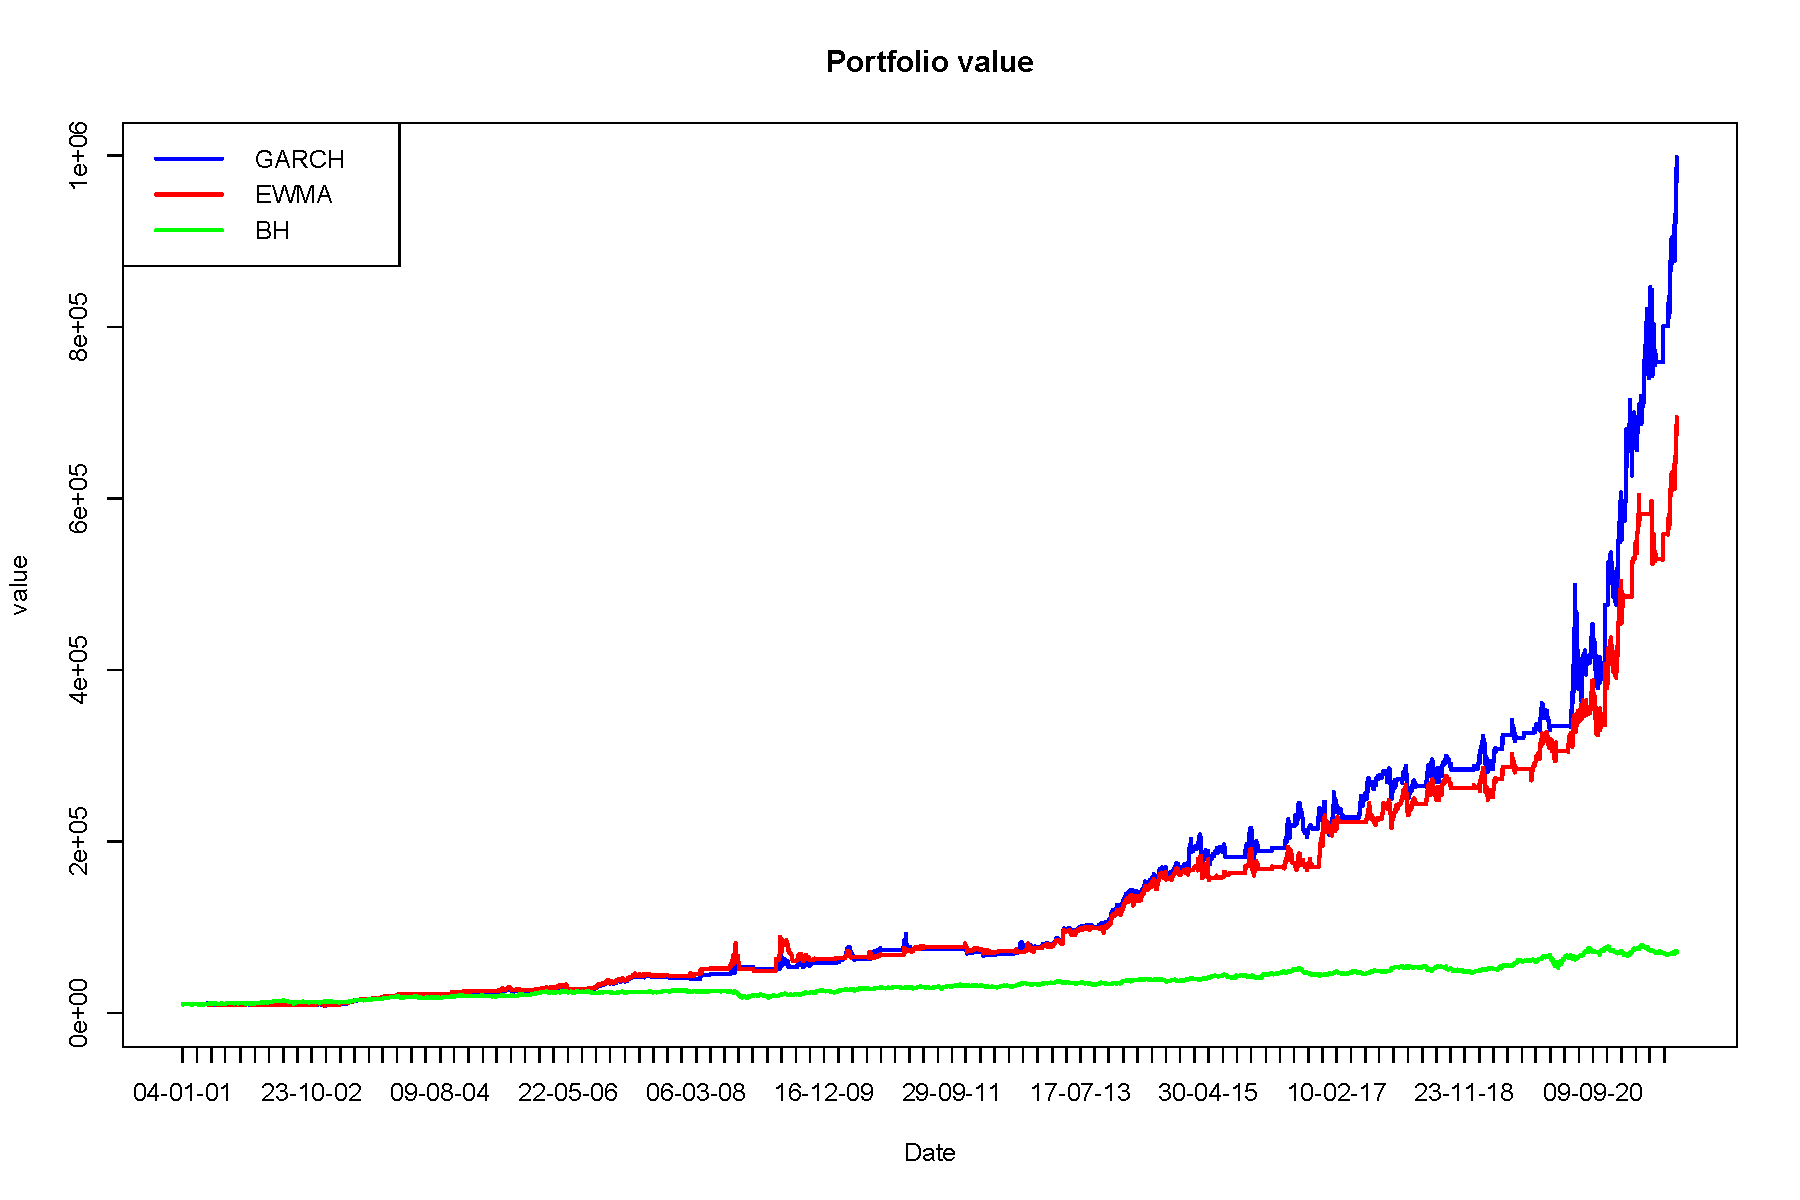
\includegraphics[width = 0.9\textwidth]{plot/PCA/1.pdf}
        \caption{Portfolio value using different approach}
        \label{fig:Fig.1}
    \end{figure}
    
    \noindent Portfolio value at last trading date: \\
    GARCH(1,1): 1486956 USD\\
    EWMA: 690605 USD\\
    Buy and Hold: 70415 USD\\
    Figure \ref{fig:Fig.1} demonstrates the  portfolio value after implementing our investment strategy and buy-and-hold our historical PCA selection in 2000. Blue line indicates our strategy using GARCH(1,1) as the volatility estimate, which outperforms the red lines using EWMA model and green lines(Buy-and Hold). Our strategy using GARCH(1,1) model has result in an around 150 times return from the principal 10000USD. While the EWMA model results in around 70 times of the principal. However Buy and Hold strategy just got 7 times of the principal.
    
 
    \begin{figure}[!ht]
        \centering
        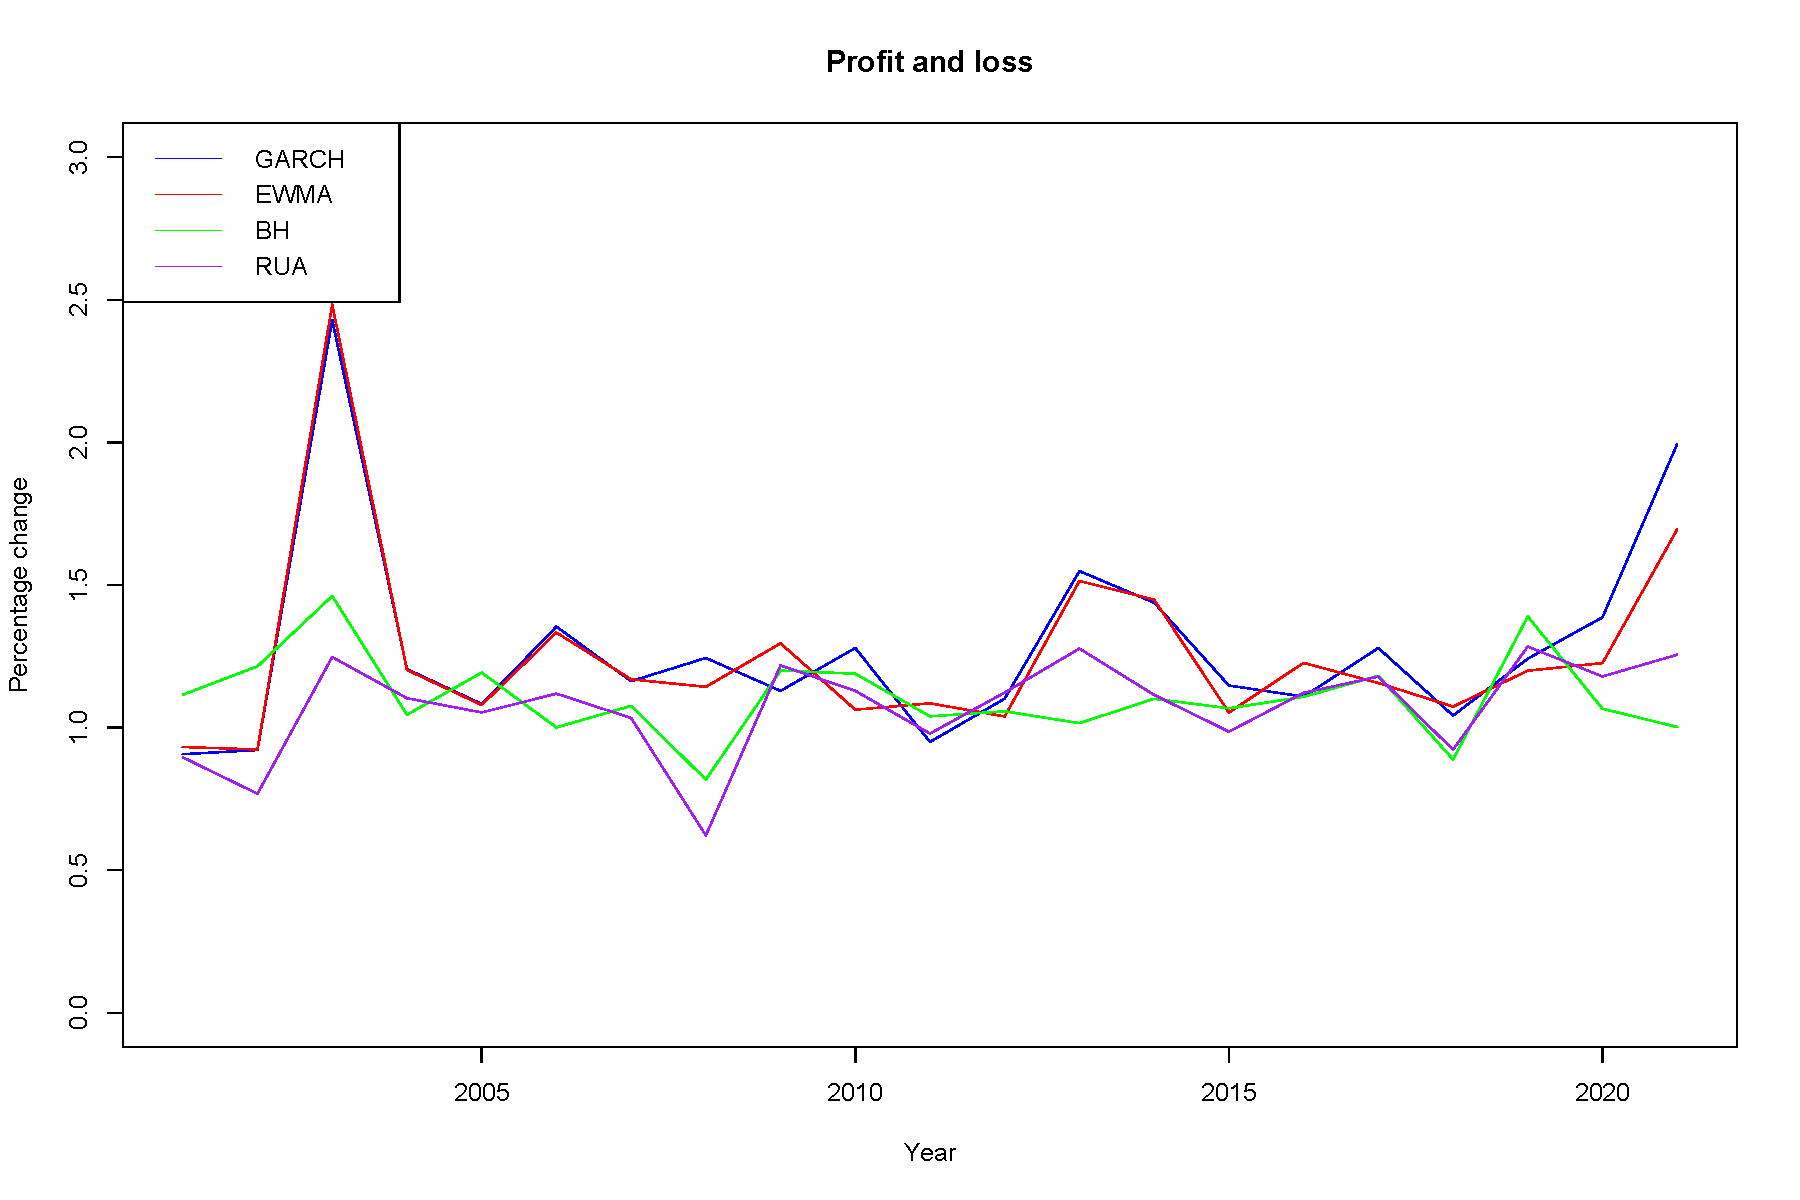
\includegraphics[width = 0.9\textwidth]{plot/PCA/2.pdf}
        \caption{Year ended profit and loss using different approach}
        \label{fig:Fig.2}
    \end{figure}
    
    \begin{table}[H]
    \centering
    \begin{tabular}{lllll}
    \hline
                              & Garch (\%) & EWMA (\%) & BH (\%) & RUA (\%) \\ \hline
    \multicolumn{1}{l|}{2001} & 90.67      & 93.19    & 111.52 & 89.58   \\
    \multicolumn{1}{l|}{2002} & 92.13      & 92.33    & 121.49 & 76.81   \\
    \multicolumn{1}{l|}{2003} & 242.91     & 248.33   & 146.12 & 124.73  \\
    \multicolumn{1}{l|}{2004} & 120.51     & 120.22   & 104.5  & 110.3   \\
    \multicolumn{1}{l|}{2005} & 108.27     & 107.93   & 119.27 & 105.3   \\
    \multicolumn{1}{l|}{2006} & 135.41     & 133.33   & 100.06 & 111.9   \\
    \multicolumn{1}{l|}{2007} & 116.26     & 116.93   & 107.62 & 103.36  \\
    \multicolumn{1}{l|}{2008} & 124.41     & 114.28   & 81.76  & 62.19   \\
    \multicolumn{1}{l|}{2009} & 112.88     & 129.55   & 119.99 & 121.79  \\
    \multicolumn{1}{l|}{2010} & 127.9      & 106.28   & 118.9  & 112.86  \\
    \multicolumn{1}{l|}{2011} & 94.97      & 108.51   & 103.95 & 97.91   \\
    \multicolumn{1}{l|}{2012} & 110.15     & 103.9    & 105.71 & 112.29  \\
    \multicolumn{1}{l|}{2013} & 154.87     & 151.42   & 101.55 & 127.69  \\
    \multicolumn{1}{l|}{2014} & 143.8      & 144.86   & 110.1  & 111.46  \\
    \multicolumn{1}{l|}{2015} & 114.76     & 105.3    & 106.76 & 98.59   \\
    \multicolumn{1}{l|}{2016} & 110.84     & 122.69   & 110.8  & 112.18  \\
    \multicolumn{1}{l|}{2017} & 127.91     & 115.64   & 118.16 & 117.88  \\
    \multicolumn{1}{l|}{2018} & 104.21     & 107.35   & 88.83  & 92.25   \\
    \multicolumn{1}{l|}{2019} & 124.17     & 119.95   & 138.97 & 128.4   \\
    \multicolumn{1}{l|}{2020} & 138.67     & 122.62   & 106.61 & 117.94  \\
    \multicolumn{1}{l|}{2021} & 199.48     & 169.52   & 100.2  & 125.55  \\ \hline
    \end{tabular}
    \caption{Year ended percentage of each trading strategy}
    \label{tab:1}
    \end{table}
    
    \newpage
    \noindent
    Figure \ref{fig:Fig.2} and Table \ref{tab:1} show the year ended percentage change for each approach. We can see that most of the year our proposed trading strategies are making profit. For GARCH(1,1), 18 out of 21 years are making profit. The losses have occurred in only 3 out of 21 years. The largest profit was +142.91\% in 2003, and the largest loss was  - 9.33\% in 2001. For EWMA, 19 out of 21 years are making profit. The losses have occurred in only 2 out of 21 years. The largest profit was +148.33\% in 2003, and the largest loss was -7.67\% in 2002. From Figure 2, we can see that most of the years the performance of our proposed trading strategies are better than buy and hold strategy and Russell3000 index. Also, they can prevent losses from the global financial crisis in 2008. The Russell3000 index loss with -37.81\% in 2008, buy and hold strategy loss with -12.24\% in 2008. However, our proposed trading strategies were making profit in 2008.
    
    
    \begin{table}[H]
    \centering
    \begin{tabular}{lll}
    \hline
    \multicolumn{3}{l}{GARCH(1,1)}                         \\
    Stocks & Trading frequency & Sector                    \\ \hline
    ATI    & 38                & Basic Materials/Resources \\
    CENX   & 36                & Basic Materials/Resources \\
    CPE    & 32                & Energy Service            \\
    CLF    & 30                & Basic Materials/Resources \\
    EMKR   & 28                & Technology                \\
    MTW    & 28                & Industrial Goods          \\
    WRLD   & 28                & Financial Services        \\
    YELL   & 28                & Logistics                 \\
    MTG    & 26                & Financial Services        \\
    GERN   & 24                & Health care               \\ \hline
    \end{tabular}
    \caption{Most frequently traded stocks using GARCH}
    \label{tab:2}
    \end{table}
    
    
    \begin{table}[H]
    \centering
    \begin{tabular}{lll}
    \hline
    \multicolumn{3}{l}{EWMA}                               \\
    Stocks & Trading frequency & Sector                    \\ \hline
    CENX   & 52                & Basic Materials/Resources \\
    MTG    & 52                & Financial Services        \\
    CLF    & 40                & Basic Materials/Resources \\
    SRPT   & 40                & Health care               \\
    ATI    & 36                & Basic Materials/Resources \\
    MTW    & 36                & Industrial Goods          \\
    SNBR   & 36                & Consumer Goods            \\
    CPE    & 32                & Energy Service            \\
    EMKR   & 32                & Technology                \\
    YELL   & 32                & Logistics                 \\ \hline
    \end{tabular}
    \caption{Most frequently traded stocks using EWMA
    }
    \label{tab:3}
    \end{table}
    
    
    \begin{table}[H]
    \centering
    \begin{tabular}{l|ll}
    \hline
               & Buy triggered & Sell triggered \\ \hline
    GARCH(1,1) & 109           & 108            \\
    EWMA       & 131           & 130            \\ \hline
    \end{tabular}
    \caption{Trading frequency}
    \label{tab:4}
    \end{table}
    
    \newpage
    \subsection{Interpretation}
    \subsubsection{Trading Frequency}
    Table \ref{tab:4} indicates that the number of trades in EWMA model is higher than GARCH(1,1) for about 30 trades, we can interpret that the goodness of using EWMA is easier to be triggered compared to GARCH(1,1). However when we are comparing the most frequent trade in Table \ref{tab:1} and \ref{tab:2}, EWMA trades about two times more than GARCH(1,1) in their most traded stocks.
    
    
    \subsubsection{Diversification}
    Table \ref{tab:2} and \ref{tab:3} highlighted the sectors of the stocks in the correspondent portfolio, the sectors of these most frequently traded stocks are diversified over the portfolio in both GARCH(1,1) and EWMA model, with various types of sectors such as Basic Materials, Technology, Energy service, Financial service, etc. The PCA method extracts the independent components from the index. The good performing stocks and the uncorrelated variables are selected by PCA. The resulting portfolio can perform as principal components of the Russell3000 index, which can be used to represent the financial market and reduce the noise and underperforming stocks.
    
    
    \subsubsection{Major Market Events}
    There were two major financial crises included in our project, i.e. during 2008 - 2009 and during 2020. They were worth mentioning as we expected our strategy to outperform even during an economic downturn. \\ \\
    The 2008 to 2009 financial crisis was mainly due to the bursting of the housing bubble in U.S.. At that time, the default rate was high due to the drop in housing prices. Therefore, we assumed that the real estate market and bank stocks would perform worse and we believed that they would be automatically excluded by our trading strategy. \\ \\
    During that period, the return of our trading strategy was 24.41\% and 14.28\% respectively of GARCH and EWMA model. At that time, our strategy had traded 8 times with PCA selected portfolio. They were mainly health care, logistics stocks  These types of stocks could perform well during the financial crisis because they are not correlated to the real estate market. \\ \\
    Simultaneously, the return of Russell3000 falls over 37\%  , much lower than our trading strategy. \\ \\
    On the other hand, the 2020 financial crisis was due to COVID-19. Because of the fear of pandemic, people were pessimistic about the economy and even some risk-free assets faced drop in prices. Therefore, we assumed that some stocks such as luxury goods, aviation, and tourism would perform worse and we believed that they would be automatically excluded by our trading strategy. \\ \\
    During 2020, the return of our trading strategy was 38\% and 22.6\% respectively. The virus affected the stock market mostly during late February to Early April, by our investment strategy, we sold all of our portfolio on 2020-02-04 and 2020-03-05 in GARCH and EWMA model while start buying on 2020-05-18 and 2020-05-04. Our strategy had dodged away the tremendous fall in the crisis and still had a positive return in the whole year. \\ \\
    Simultaneously, the return of buy-and-hold Russell3000 was only 18\%, much lower than our trading strategy. \\ \\
    In short, the simulation proved that our trading strategy, which is a combination of PCA, portfolio optimization, and Kelly's Formula, performs better than the market, no matter whether the economy is in upturn or in downturn.
    
    
    \newpage
    \subsection{Conclusion}
    In this project, we introduce a stock selection method with PCA, a portfolio weighting method with Mean-Variance optimization method, and a trading strategy with Kelly's formula using GARCH model and EWMA method for forecasting. These three techniques combined together to form an optimal trading strategy to compare with buy and hold strategy and Russell3000 index. The testing period is between 2001-01-04 and 2021-11-12. The trading strategy we proposed can outperform the Russell3000 index and buy and hold strategy in the testing period.
    
    
    \subsubsection{Limitations}
    \begin{enumerate}
    \item We proposed that we triggered the buy/sell signal by the threshold that is determined by the overall portfolio return and volatility, if one of the stocks in the portfolio performs badly, we might not able to notice that and change our portfolio
    
    \item Due to the large data size, the total running time of the simulation was long. Meanwhile, since we run through all the trading days with GARCH(1,1) and EWMA,  the for-loops in the program have further lengthened the running time.
    
    \item In our project, we downloaded all required data first then did the simulation. However, in practice, data may need to be updated daily. It is daily additional work and time is needed to download all the components’ price in Russell300 to start the analysis every day.
    
    \item Liquidity,  the simulation assumed that stock could be bought or sold immediately. But in the real world, there may be a time lag for the trading to be done, especially if the trading volume for that stock is not high. This may result in a reduction of return as price may have changed during the time lag. On the contrary, the buy-and-hold strategy would not have this problem because it only buys or sells once in the trading period.
    \end{enumerate}
    
    
    \subsubsection{Improvements}
    \begin{enumerate}
    \item To shorten the running time in practice, we could choose only one among the GARCH(1,1) and EWMA volatility estimation methods. From the simulation, we could see that the portfolio return calculated by GARCH(1,1) and EWMA had very similar results from the start of the simulation period to the end of it.
    
    \item The number of stocks in the pool could be smaller. In our simulation, we picked all components of Russell3000 into the pool for PCA. In practice, however, we may choose fewer stocks to put into the pool. This could shorten the time for data collection and extraction. It is suggested that the market value of stocks to be not too small, for example at least greater than 1 billion, and that the pool should contain various types of stocks so that the strategy would be able to cater different economic situations. It is important to note that since the pool is smaller, maybe we need to update the stocks in the pool regularly for more accurate results. There are trade-offs between accuracy and data set size.
    
    \item To lower the chance that the stock is too hard to be traded due to a small trading volume in the market, we may avoid choosing less popular stocks.
    
    \item Short Selling can be considered to be added to the strategy by selecting the least loadings in the PCA computed, also as our buy/sell strategy is based on volatility, short selling can also be possible in our strategy.
    \end{enumerate}
    
    
    % Section 2
    \newpage
    \section{Classification / Decision and Regression Trees}
    \textbf{This section is contributed by LAM Wai Chui (SID: 1155152095) and LAW Yiu Leung Eric (SID: 1155149315)}. \\
    In this section, we are going to use Decision Tree and Random Forest methods to predict binary response variable. The source code is attached in \texttt{src/python/classification.ipynb}, notice that the output in this written report may be slightly different with the python notebook, due to random seed is involved.
    
    \subsection{Dataset}
    For the dataset, we use \href{https://archive.ics.uci.edu/ml/datasets/bank+marketing}{Bank Marketing Data Set} from  \href{https://archive.ics.uci.edu/ml/index.php}{UCI Machine Learning Repository}.
    The data is related with direct marketing campaigns of a Portuguese banking institution. The marketing campaigns were based on phone calls. Often, more than one contact to the same client was required, in order to access if the product (bank term deposit) would be ('yes') or not ('no') subscribed \cite{MORO201422}. There are total 21 variables (including y, the response variable), 41188 valid records. \\
    
    \noindent
    \textbf{Samples of the dataset:}
    \begin{table}[ht]
        \centering
        \begin{tabular}{lrlllllllcl}
            {} &  age &          job &   marital &          education & default & housing & loan &   contact & ... & y\\
            
            \hline \hline
            
            35666 &   58 &   management &   married &  university.degree &      no &      no &   no &  cellular & ... & no \\
            36531 &   48 &       admin. &   married &  university.degree &      no &     yes &   no &  cellular & ... & yes \\
            38676 &   73 &      retired &   married &  university.degree &      no &      no &  yes &  cellular & ... & yes \\
            15146 &   49 &   technician &  divorced &        high.school &      no &      no &   no &  cellular & ... & no \\
            33230 &   33 &  blue-collar &    single &           basic.6y &      no &     yes &   no &  cellular & ... & no \\
        \end{tabular} \\ \\
        \caption{Dataset Samples}
        \label{tab:samples}
    \end{table}
    
    \noindent
    There are 41188 observations with 21 features
    % \begin{tabular}{lrlllllllcl}
    %     {} &  age &          job &   marital &          education & default & housing & loan &   contact & ... & y\\
        
    %     35666 &   58 &   management &   married &  university.degree &      no &      no &   no &  cellular & ... & no \\
    %     36531 &   48 &       admin. &   married &  university.degree &      no &     yes &   no &  cellular & ... & yes \\
    %     38676 &   73 &      retired &   married &  university.degree &      no &      no &  yes &  cellular & ... & yes \\
    %     15146 &   49 &   technician &  divorced &        high.school &      no &      no &   no &  cellular & ... & no \\
    %     33230 &   33 &  blue-collar &    single &           basic.6y &      no &     yes &   no &  cellular & ... & no \\
    % \end{tabular} \\ \\
    % There are 41188 observations with 21 features
    
    
    \subsection{Feature Description}
    There are 20 explanatory variables, including numerical and categorical variables:
    
    \begin{table}[h]
        \begin{minipage}{.5\linewidth}
            \centering
            \begin{tabular}{r c c}
                 & Feature & Type \\
                \hline \hline
                \rownumber & age & numerical \\
                \rownumber & job & categorical \\
                \rownumber & marital & categorical \\
                \rownumber & education & categorical \\
                \rownumber & default & categorical \\
                \rownumber & housing & categorical \\
                \rownumber & loan & categorical \\
            \end{tabular}
            \caption{Bank client data}\label{tab:bank.client}
        \end{minipage}%
        \begin{minipage}{.5\linewidth}
            \centering
            \begin{tabular}{r c c}
                 & Feature & Type \\
                \hline \hline
                \rownumber & contact & categorical \\
                \rownumber & month & categorical \\
                \rownumber & day\_of\_week & categorical \\
                \rownumber & duration & numerical \\
            \end{tabular}
            \caption{Related with the last contact of the current campaign}\label{tab:last.contact}
        \end{minipage}
    \end{table}
    
    \begin{table}[h]
        \begin{minipage}{.5\linewidth}
            \centering
            \begin{tabular}{r c c}
                 & Feature & Type \\
                \hline \hline
                \rownumber & campaign & numerical \\
                \rownumber & pdays & numerical \\
                \rownumber & previous & numerical \\
                \rownumber & poutcome & categorical \\
            \end{tabular}
            \caption{Other attributes}\label{tab:other}
        \end{minipage}%
        \begin{minipage}{.5\linewidth}
            \centering
            \begin{tabular}{r c c}
                 & Feature & Type \\
                \hline \hline
                \rownumber & emp.var.rate & numerical \\
                \rownumber & cons.price.idx & numerical \\
                \rownumber & cons.conf.idx & numerical \\
                \rownumber & euribor3m & numerical \\
                \rownumber & nr.employed & numerical \\
            \end{tabular}
            \caption{social and economic context attributes}\label{tab:soc.econ}
        \end{minipage}
    \end{table}
    
    \newpage
    \subsection{Project Description}
    We are going to perform an analysis in \textbf{topic 6: Classification / Decision and Regression Trees}. We will use \nameref{decision_trees}, \nameref{random_forest} and also \nameref{logistic_regression} to do classification on response variable \textbf{y}, i.e. whether the client subscribed a term deposit. \\
    
    
    \noindent
    The following steps will be performed to complete this section:
    \begin{enumerate}
        \item process data explanatory data analysis (EDA)
        \item data preparation for modeling
        \item visualization of random forest, decision tree and logistic regression
        \item cross validation and grid search
        \item logistic regression
        \item comparison of performance of random forest, decision tree and logistic regression
        \item conclusion
    \end{enumerate}
    
    \subsection{Process Data and Explanatory Data Analysis (EDA)}
%     Import libraries
% \begin{lstlisting}[language = Python]
% import pandas as pd
% import numpy as np
% from datetime import datetime
% import time
% import gc
% from IPython.display import display
% import warnings
% warnings.filterwarnings("ignore")

% from sklearn.model_selection import train_test_split, GridSearchCV, StratifiedKFold
% from sklearn.ensemble import RandomForestClassifier
% from sklearn import tree
% from sklearn.pipeline import Pipeline
% from sklearn.metrics import roc_curve, roc_auc_score
% import category_encoders as ce

% import plotly.graph_objs as go
% import matplotlib.pyplot as plt
% \end{lstlisting}

    % \noindent
    In order to easily implement machine learning algorithms, instead of writing from scratch, we imported \texttt{sklearn} library \cite{sklearn_api}.
    
%     \noindent Loading data and a short explanatory data analysis
% \begin{lstlisting}[language = Python]
% # Process data
% data = pd.read_csv('../../data/bank-additional-full.csv', sep=';')
% display(data.sample(10))
% display('There are {} observations with {} features'.format(data.shape[0], data.shape[1]))
% \end{lstlisting}
    
    
    
    \subsubsection{Categorical Variables}
% \begin{lstlisting}[language = Python]
% # Function of plotting the categorical values disribution
% def plot_bar(column):
%     temp = pd.DataFrame()  #create a tremp dataframe
%     temp['Not_deposit'] = data[data['y'] == 'no'][column].value_counts() # count the value when y = no
%     temp['Deposit'] = data[data['y'] == 'yes'][column].value_counts() # count the value when y = yes

%     temp = temp.apply(lambda x: x / x.sum(), axis = 1) * 100
%     temp.sort_values("Deposit", inplace = True)
%     temp.plot(
%         kind = "barh", 
%         stacked = True, 
%         title = "Percentage Stacked Bar Graph for {}".format(column), 
%         mark_right = True
%     ).legend(loc = "center left", bbox_to_anchor = (1, 0.5))

%     plt.savefig("../../plot/classification/{}.pdf".format(column), bbox_inches = "tight")
%     plt.show();

% plot_bar('job'), plot_bar('marital'), plot_bar('education'), plot_bar('contact'), plot_bar('loan'), plot_bar('housing')
% \end{lstlisting}
    
    We plot percentage stacked bar graphs for 6 categorical variables in table \ref{tab:bank.client} vs. \texttt{y}, to see the proportions of \texttt{y} = 1 given the client is different categories.
    
    \noindent
    \begin{figure}[H]
        \centering
        \subfloat[job]{\includegraphics[scale=0.45]{plot/classification/eda/job.pdf}}%
        \qquad
        \subfloat[marital]{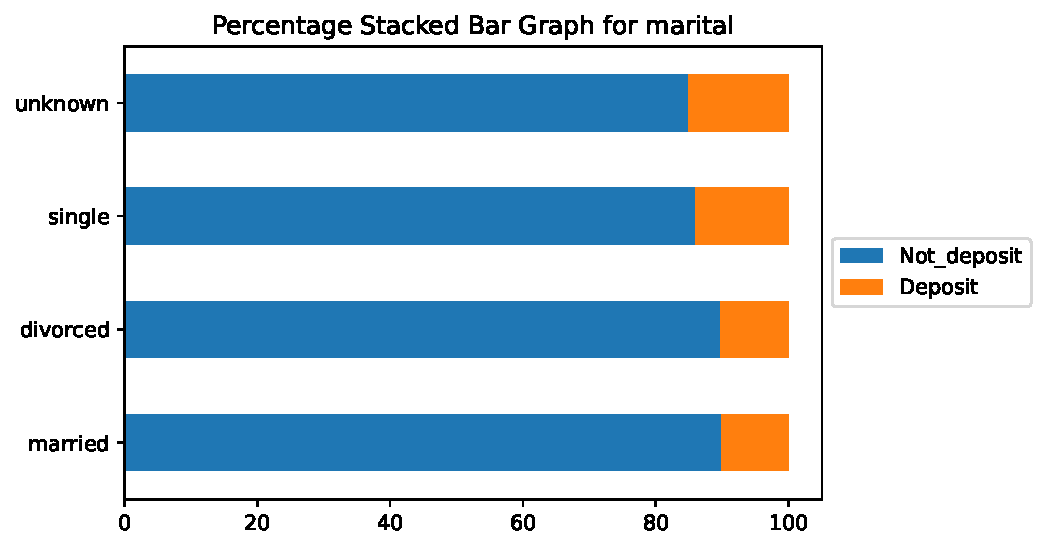
\includegraphics[scale=0.45]{plot/classification/eda/marital.pdf}}%
    
        \subfloat[education]{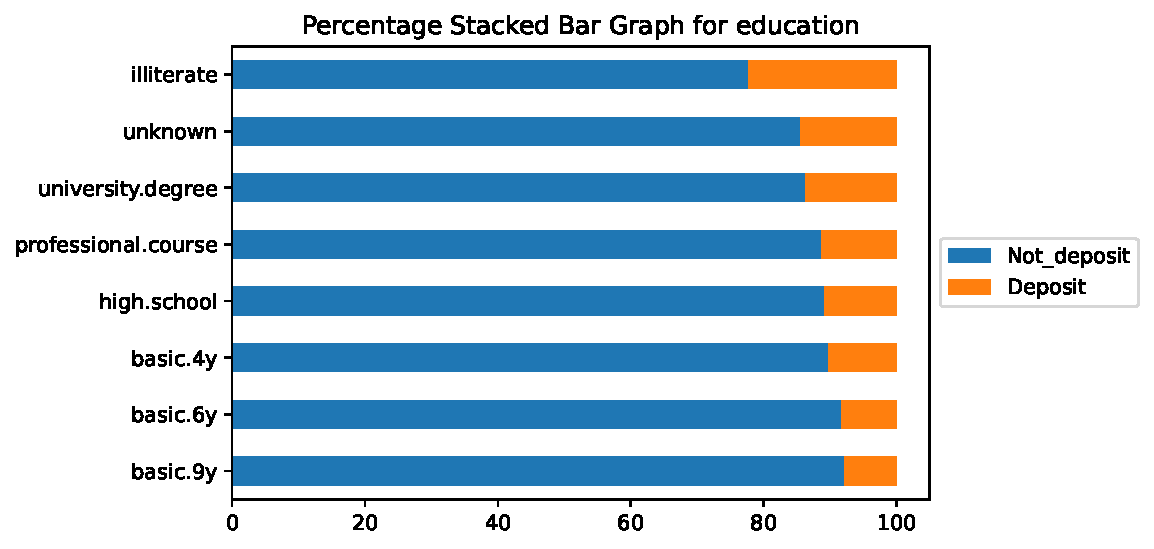
\includegraphics[scale=0.45]{plot/classification/eda/education.pdf}}%
        \qquad
        \subfloat[contact]{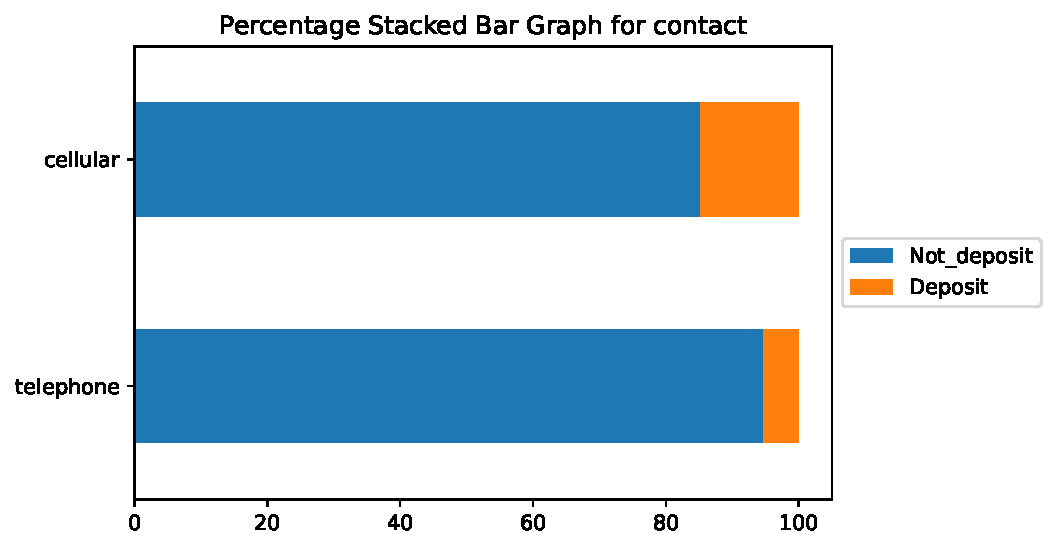
\includegraphics[scale=0.45]{plot/classification/eda/contact.pdf}}%
        
        % \subfloat[loan]{\includegraphics[scale=0.4]{plot/classification/loan.pdf}}%
        % \qquad
        % \subfloat[contact]{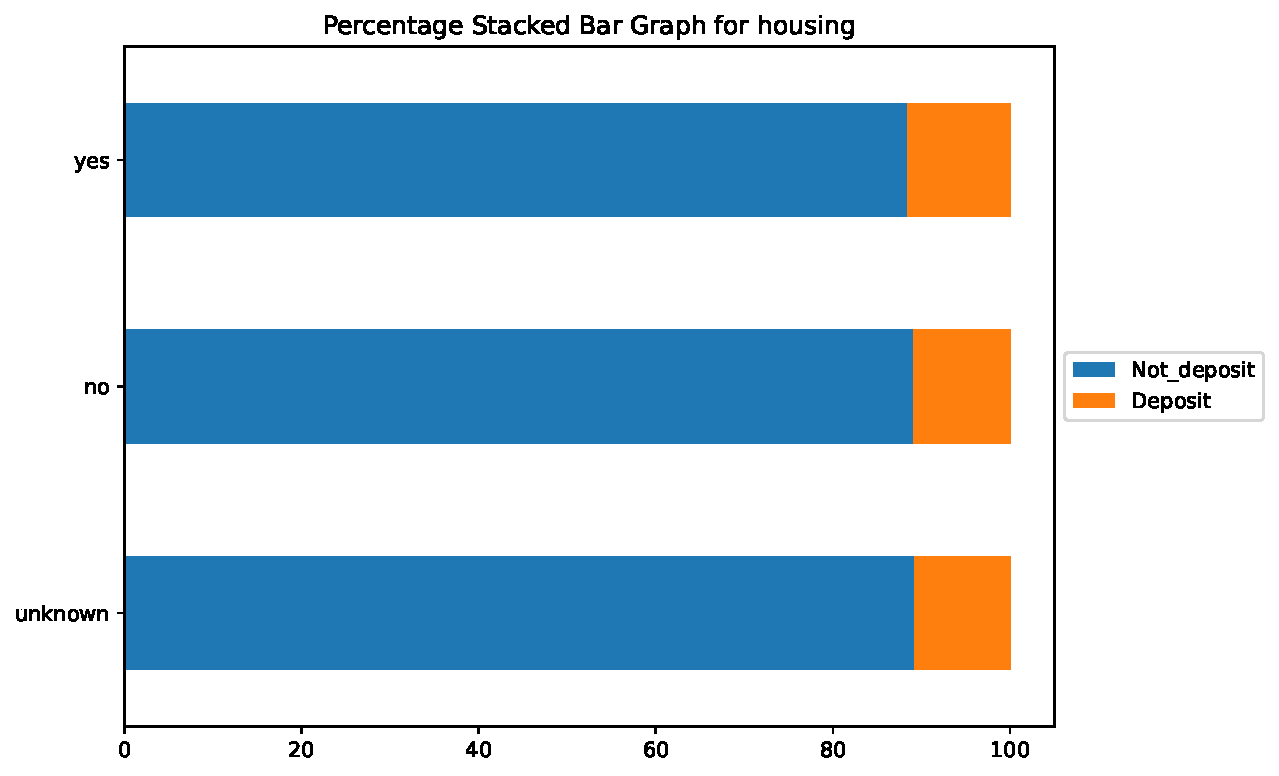
\includegraphics[scale=0.4]{plot/classification/housing.pdf}}%
    \end{figure}
    
        \begin{figure}[H]
        \centering
        % \subfloat[job]{\includegraphics[scale=0.4]{plot/classification/job.pdf}}%
        % \qquad
        % \subfloat[marital]{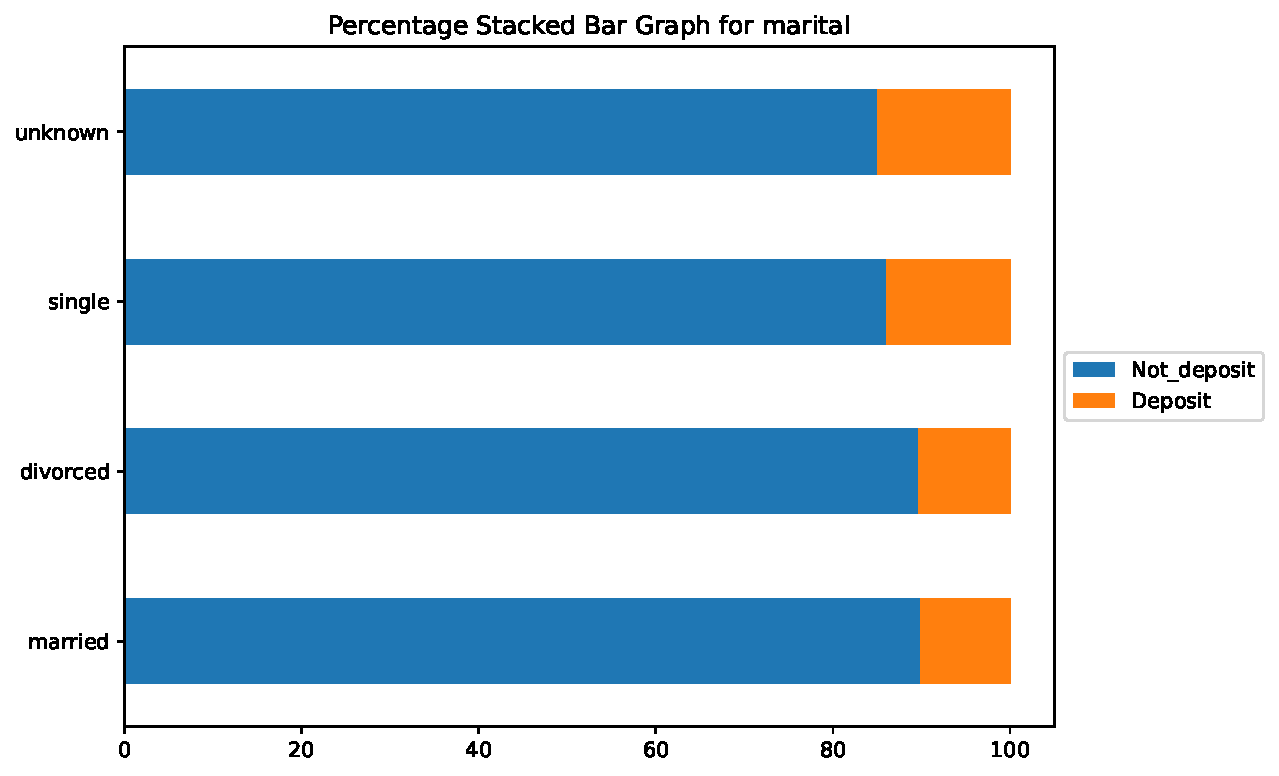
\includegraphics[scale=0.4]{plot/classification/marital.pdf}}%
    
        % \subfloat[education]{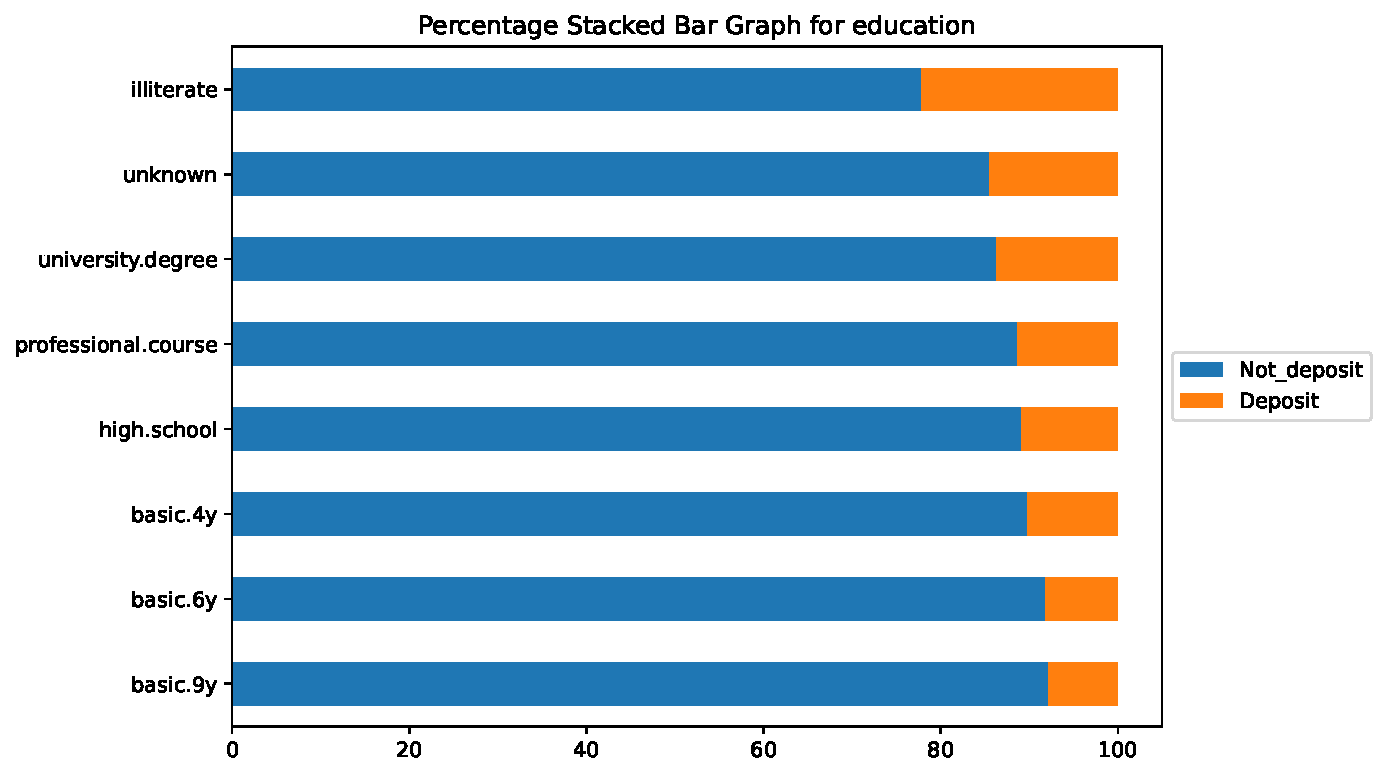
\includegraphics[scale=0.4]{plot/classification/education.pdf}}%
        % \qquad
        % \subfloat[contact]{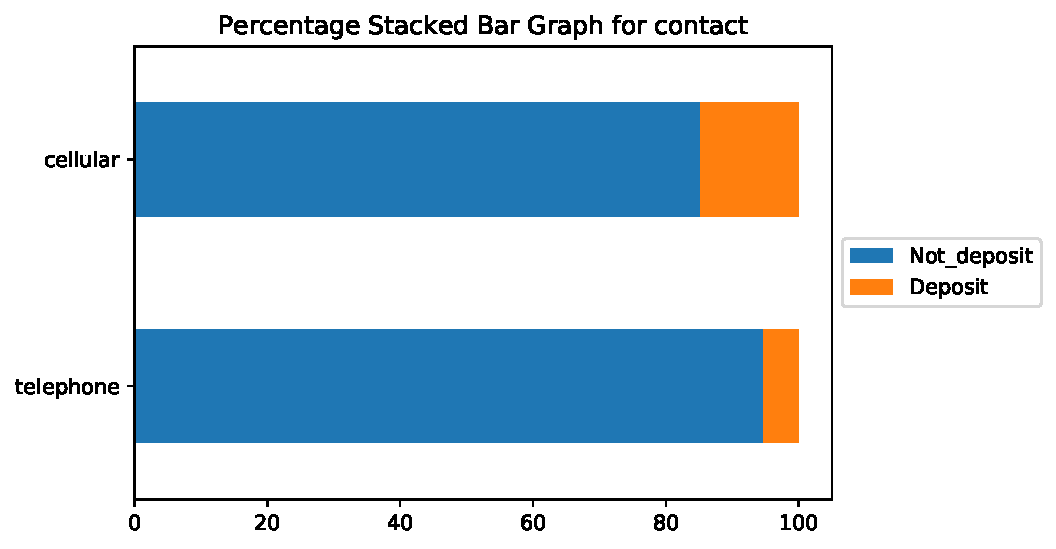
\includegraphics[scale=0.4]{plot/classification/contact.pdf}}%
        
        \subfloat[loan]{\includegraphics[scale=0.45]{plot/classification/eda/loan.pdf}}%
        \qquad
        \subfloat[contact]{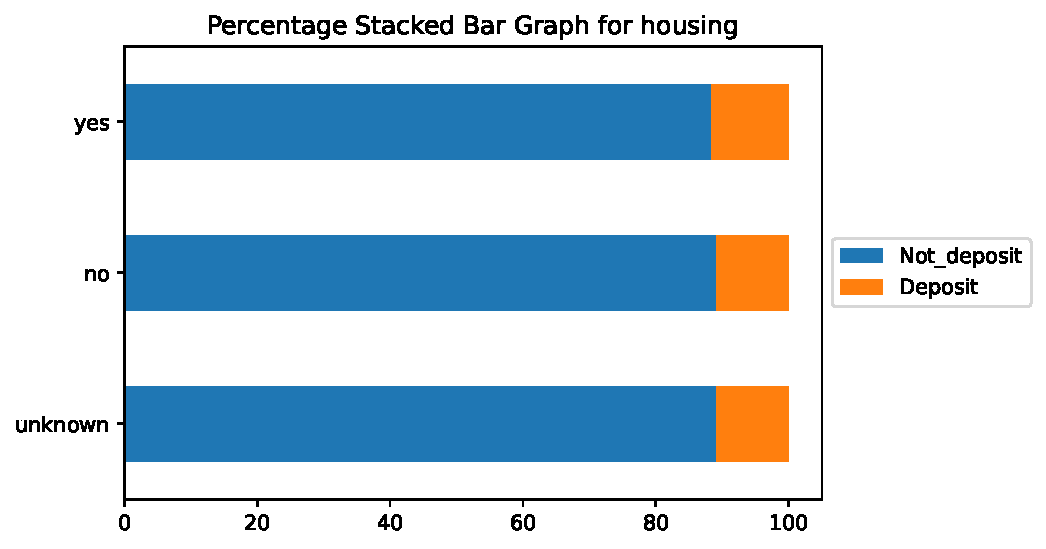
\includegraphics[scale=0.45]{plot/classification/eda/housing.pdf}}%
    \end{figure}
    
    
    
    \noindent \textbf{Summary of Categorical Variables:}
    \begin{enumerate}
        \item 
            The proportion of opening deposit or not is different among different job type. When the job types are student, retired and unemployed, the proportions of opening the deposit are highest. When the job types are entrepreneur, services and blue-collar, the proportions of opening the deposit are lowest.
        
        \item
            The proportion of opening deposit of unknown is close to that of single, while both of them have higher proportion than divorced and married.
        
        \item
            It is surprised to see that illiterate has the highest proportion, other than that, generally higher education levels have higher proportion of opening deposit.
            
        \item
            The proportion of opening deposit of using cellular is much higher than that of using telephone.
            
        \item
            The proportion is basically no different among loan status.
            
        \item
            The proportion is basically no different among contact status.
    \end{enumerate}
    
    \subsubsection{Numerical Variables}
% \begin{lstlisting}[language = Python]
% corr = data.corr()
% corr.style.background_gradient(cmap = 'Spectral')
% \end{lstlisting}
    After exploring the categorical variables, we take a look into numerical variables, by calculate (Pearson) correlations of each variables, we can see which variables have significant relationship with \texttt{y}. The correlation matrix are as follow: 
    \begin{table}[h]
        \centering
        {\tiny
            \begin{tabular}{l||rrrrrrrrrrr}
                {} &     age &  duration &  campaign &   pdays &  previous &  emp.var.rate &  cons.price.idx &  cons.conf.idx &  euribor3m &  nr.employed &       y \\
                \hline \hline
                age            &  1.0000 &   -0.0009 &    0.0046 & -0.0344 &    0.0244 &       -0.0004 &          0.0009 &         0.1294 &     0.0108 &      -0.0177 &  0.0304 \\
                duration       & -0.0009 &    1.0000 &   -0.0717 & -0.0476 &    0.0206 &       -0.0280 &          0.0053 &        -0.0082 &    -0.0329 &      -0.0447 &  0.4053 \\
                campaign       &  0.0046 &   -0.0717 &    1.0000 &  0.0526 &   -0.0791 &        0.1508 &          0.1278 &        -0.0137 &     0.1351 &       0.1441 & -0.0664 \\
                pdays          & -0.0344 &   -0.0476 &    0.0526 &  1.0000 &   -0.5875 &        0.2710 &          0.0789 &        -0.0913 &     0.2969 &       0.3726 & -0.3249 \\
                previous       &  0.0244 &    0.0206 &   -0.0791 & -0.5875 &    1.0000 &       -0.4205 &         -0.2031 &        -0.0509 &    -0.4545 &      -0.5013 &  0.2302 \\
                emp.var.rate   & -0.0004 &   -0.0280 &    0.1508 &  0.2710 &   -0.4205 &        1.0000 &          0.7753 &         0.1960 &     0.9722 &       0.9070 & -0.2983 \\
                cons.price.idx &  0.0009 &    0.0053 &    0.1278 &  0.0789 &   -0.2031 &        0.7753 &         1.0000 &         0.0590 &     0.6882 &       0.5220 & -0.1362 \\
                cons.conf.idx  &  0.1294 &   -0.0082 &   -0.0137 & -0.0913 &   -0.0509 &        0.1960 &          0.0590 &         1.0000 &     0.2777 &       0.1005 &  0.0549 \\
                euribor3m      &  0.0108 &   -0.0329 &    0.1351 &  0.2969 &   -0.4545 &        0.9722 &          0.6882 &         0.2777 &     1.0000 &       0.9452 & -0.3078 \\
                nr.employed    & -0.0177 &   -0.0447 &    0.1441 &  0.3726 &   -0.5013 &        0.9070 &          0.5220 &         0.1005 &     0.9452 &       1.0000 & -0.3547 \\
                y              &  0.0304 &    0.4053 &   -0.0664 & -0.3249 &    0.2302 &       -0.2983 &         -0.1362 &         0.0549 &    -0.3078 &      -0.3547 &  1.0000 \\
            \end{tabular}
        }
        \caption{Correlation Matrix}
        \label{tab:corr_mat}
    \end{table}

    \noindent
    \textbf{Summary of Numerical Variables:}
    \begin{itemize}
        \item \texttt{duration} is the highest correlated variable with target feature (0.4053).
        \item \texttt{nr.employed, pdays, euribor3m} are also highly correlated with target feature.
    \end{itemize}
    
    
    \newpage
    \subsection{Data Preparation for modeling}
    \subsubsection{Transformation for Categorical Variables}
    Since this dataset contains a lot of categorical variables and the number of weakly correlated numeric variables is small, therefore, we use one-hot encoding to transform categorical data.
    \begin{itemize}
        \item 
            For binary categorical variables (\texttt{"yes", "no"}), we transform it into binary number accordingly (\texttt{0, 1}).
            
        \item
            For \texttt{job, marital, education, month, day\_of\_week}, we use one-hot encoding to transform these variables since they have more than 3 types of possible options. Also, some variables contain missing data, labeled as \texttt{unknown} or \texttt{nonexistent}, we treat it as 0 (i.e. no) in general.
        
        \item
            For \texttt{pdays}, there exists many records of \texttt{999} which means the client was not previously contacted, we replaces those with \texttt{0}.
        
        \item
            At last, we remove duplicated records.
    \end{itemize}

    
    
% \begin{lstlisting}[language = Python]
% # Fucntion of One Hot Encoding
% def encode(data, col):
%     return pd.concat([data, pd.get_dummies(col, prefix=col.name)], axis=1)

% # Replacing values with binary number
% data.contact = data.contact.map({'cellular': 0, 'telephone': 1}).astype('uint8') 
% data.loan = data.loan.map({'unknown': 0, 'no' : 0, 'yes': 1}).astype('uint8')
% data.default = data.default.map({'unknown': 0,'no': 0, 'yes': 1}).astype('uint8')
% data.housing = data.housing.map({'unknown': 0, 'no' : 0,'yes': 1}).astype('uint8')
% # binary if were was an outcome of marketing campane
% data.poutcome = data.poutcome.map({'nonexistent':0, 'failure':0, 'success':1}).astype('uint8') 

% # One Hot encoding of 3 variable 
% data = encode(data, data.job)
% data = encode(data, data.month)
% data = encode(data, data.day_of_week)

% # Drop tranfromed features
% data.drop(['job','month', 'day_of_week'], axis=1, inplace=True)

% '''Drop the dublicates'''
% data.drop_duplicates(inplace=True) 

% # Save target variable as y
% y = data.y
% # Create target encoder object and transoform marital and education
% target_encode = ce.target_encoder.TargetEncoder(cols=['marital', 'education']).fit(data, y)
% dataset_prepared = target_encode.transform(data)
% # Drop target variable
% dataset_prepared.drop('y', axis=1, inplace=True)

% display(dataset_prepared.sample(10))
% display('There are {} observations with {} features in the prepared dataset'.format(dataset_prepared.shape[0], dataset_prepared.shape[1]))
% \end{lstlisting}
    % \noindent
    \begin{table}[ht]
        \centering
        \begin{tabular}{lrrrrrrrrrc}
            {} &  age &   marital &  education &  default &  housing &  loan &  contact &  duration &  campaign & \dots \\
            \hline \hline
            29851 &   52 &  0.103231 &   0.137219 &        0 &        1 &     0 &        1 &        70 &         4 & \dots \\
            15768 &   39 &  0.140090 &   0.113550 &        0 &        0 &     0 &        0 &        65 &         2 & \dots \\
            38033 &   76 &  0.101569 &   0.102515 &        0 &        1 &     0 &        0 &       259 &         2 & \dots \\
            27290 &   37 &  0.140090 &   0.137219 &        0 &        1 &     1 &        0 &       661 &         1 & \dots \\
            30685 &   34 &  0.101569 &   0.078246 &        0 &        1 &     0 &        0 &       332 &         1 & \dots \\
        \end{tabular}
        \caption{Dataset Samples after Encoding}
        \label{tab:samples_encoded}
    \end{table}
    
    \noindent
    After removing duplicates, there are 41173 observations with 44 features in the prepared dataset
    
    
    \subsubsection{Splitting Training Dataset and Testing Dataset}
    To test the performance of machine learning alogrithm, we split the dataset into training and testing datasets, 80\% and 20\% of the full dataset respectively. The models would be built using training dataset, and evaluated the performance using testing dataset accordingly. In order to make the prediction model reproducible, we fixed the random seed: \texttt{random\_state=4002}. \\
    Total records in training dataset = 32938, number of class \texttt{0} and \textt{1} in training dataset: \texttt{[29267, 3671]}, noted that this is the numbers of true positive and true negative. These are used to calculate the support, confidence and capture in evaluating performance under training dataset.
% \begin{lstlisting}[language = Python]
% # Set global random seed
% random_state = 4002
% # split data
% x_train, x_test, y_train, y_test = train_test_split(dataset_prepared, y, test_size=0.2, random_state=random_state)
% \end{lstlisting}
    
    
    \newpage
    \subsection{Decision Tree} \label{decision_trees}
    We set the depth of decision tree to 3, in order to plot a simplified decision tree.
% \begin{lstlisting}[language = Python]
% # Set max_depth = 3 to keep the size of the tree small for ploting graph
% dt = tree.DecisionTreeClassifier(max_depth=3, random_state=random_state)
% dt.fit(x_train, y_train)
% plt.figure(figsize=(10, 5))
% _ = tree.plot_tree(dt, feature_names=dataset_prepared.columns,
%                   class_names=["0", "1"], filled=True)
% \end{lstlisting}

    % \noindent
    \begin{figure}[ht]
        \centering
        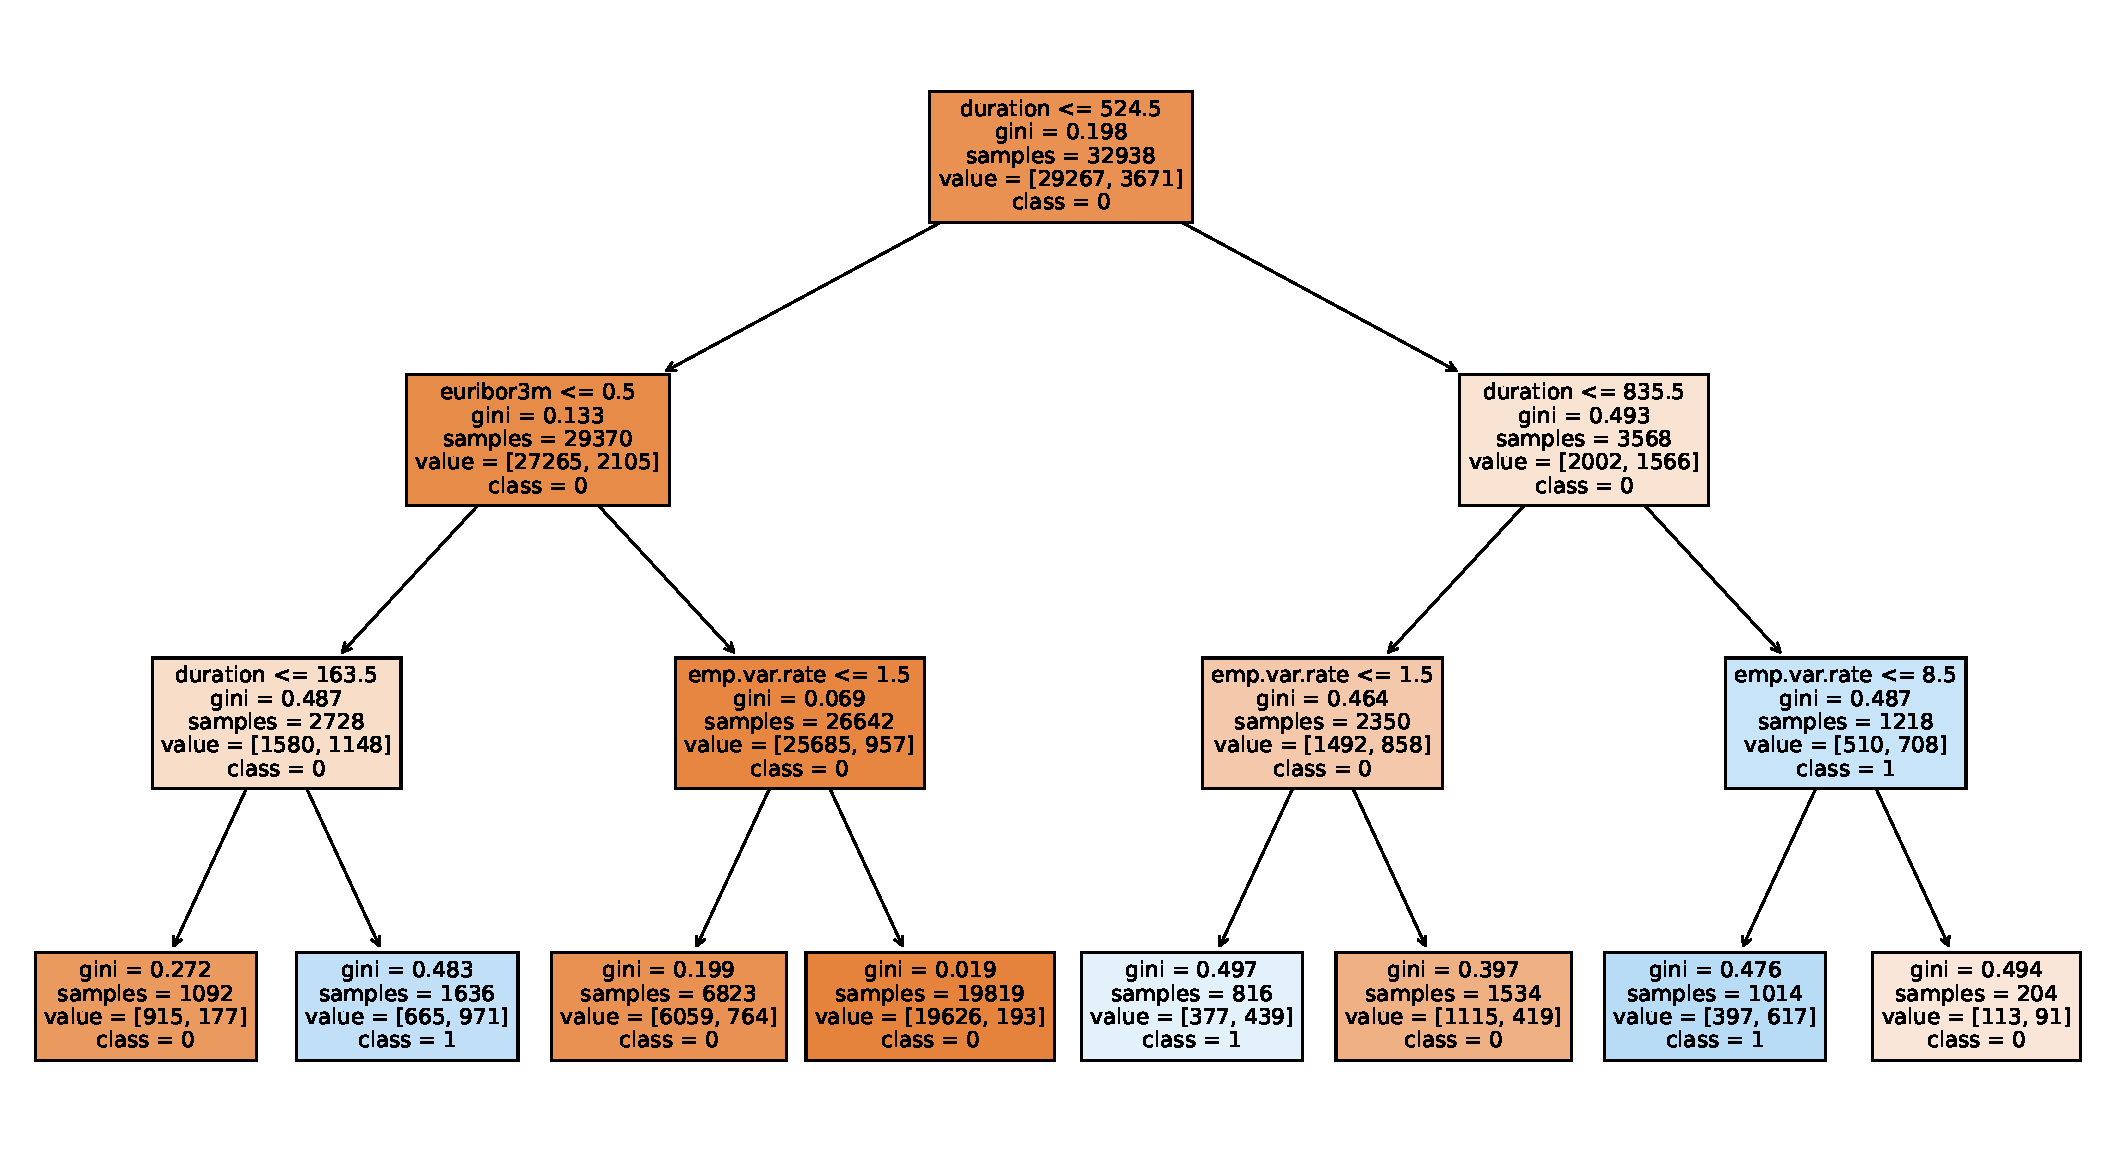
\includegraphics[width=\textwidth]{plot/classification/decision_tree.pdf}
        \caption{Decision Tree}
        \label{fig:decision_tree}
    \end{figure}

    
    % \newpage
    \noindent
    \textbf{Decision Rules} \\
    {
% \begin{lstlisting}[language = Python]
% r = tree.export_text(dt, feature_names=list(dataset_prepared.columns))
% print(r)

% |--- nr.employed <= 5087.65
% |   |--- duration <= 162.50
% |   |   |--- duration <= 123.50
% |   |   |   |--- class: 0
% |   |   |--- duration >  123.50
% |   |   |   |--- class: 0
% |   |--- duration >  162.50
% |   |   |--- pdays <= 15.50
% |   |   |   |--- class: 1
% |   |   |--- pdays >  15.50
% |   |   |   |--- class: 1
% |--- nr.employed >  5087.65
% |   |--- duration <= 524.50
% |   |   |--- cons.conf.idx <= -46.65
% |   |   |   |--- class: 0
% |   |   |--- cons.conf.idx >  -46.65
% |   |   |   |--- class: 0
% |   |--- duration >  524.50
% |   |   |--- duration <= 835.50
% |   |   |   |--- class: 0
% |   |   |--- duration >  835.50
% |   |   |   |--- class: 1
% \end{lstlisting}
        
    }

    \setcounter{magicrownumbers}{0}
    \newcommand\rules{\stepcounter{magicrownumbers}\arabic{magicrownumbers}}
    \begin{tabular}{r l}
        R\rules & If \texttt{duration} $<$= 524.5 and \texttt{euribor3m} $<$= 0.5 and \texttt{duration} $<$= 163.5, then \texttt{y} = 0 \\
        & Gini = 0.272, Support = 0.0332, Confidence = 0.8379, Capture = 0.0313 \\
        
        R\rules & If \texttt{duration} $<$= 524.5 and \texttt{euribor3m} $<$= 0.5 and \texttt{duration} $>$ 163.5, then \texttt{y} = 1 \\
        & Gini = 0.483, Support = 0.0497, Confidence = 0.5935, Capture = 0.2645 \\
        
        R\rules & If \texttt{duration} $<$= 524.5 and \texttt{euribor3m} $>$ 0.5 and \texttt{emp.var.rate} $<$= 1.5, then \texttt{y} = 0 \\
        & Gini = 0.199, Support = 0.2071, Confidence = 0.8880, Capture = 0.2070 \\
        
        R\rules & If \texttt{duration} $<$= 524.5 and \texttt{euribor3m} $>$ 0.5 and \texttt{emp.var.rate} $>$ 1.5, then \texttt{y} = 0 \\
        & Gini = 0.019, Support = 0.6017, Confidence = 0.9902, Capture = 0.6706\\
        
        R\rules & If \texttt{duration} $>$ 524.5 and \texttt{duration} $<$= 835.5 and \texttt{emp.var.rate} $<$= 1.5, then \texttt{y} = 1 \\
        & Gini = 0.497, Support = 0.0247, Confidence = 0.5380, Capture = 0.1196 \\
        
        R\rules & If \texttt{duration} $>$ 524.5 and \texttt{duration} $<$= 835.5 and \texttt{emp.var.rate} $>$ 1.5, then \texttt{y} = 0 \\
        & Gini = 0.397, Support = 0.0466, Confidence = 0.7269, Capture = 0.0381 \\
        
        R\rules & If \texttt{duration} $>$ 524.5 and \texttt{duration} $>$ 835.5 and \texttt{emp.var.rate} $<$= 8.5, then \texttt{y} = 1 \\
        & Gini = 0.476, Support = 0.0308, Confidence = 0.6085, Capture = 0.1681 \\
        
        R\rules & If \texttt{duration} $>$ 524.5 and \texttt{duration} $>$ 835.5 and \texttt{emp.var.rate} $>$ 8.5, then \texttt{y} = 0 \\
        & Gini = 0.494, Support = 0.0062, Confidence = 0.5539, Capture = 0.0039 \\
        
    \end{tabular} \\ \\
    As the maximum depth is set to be only 3, there are only 8 rules, and quite a few redundant leafs, e.g., R3 and R4 could be combined into one rule: If \texttt{duration} $<$= 524.5 and \texttt{euribor3m} $>$ 0.5, then \texttt{y} = 0
    
    \newpage
    \subsection{Random Forest} \label{random_forest}
    Again, the depth of decision trees are set to be 3, a simplified random forest is as followed:
    
% \begin{lstlisting}[language = Python]
% # Set max_depth = 3 to keep the size of the tree small for ploting graph
% rf = RandomForestClassifier(max_depth = 3, n_estimators = 10,
%                             random_state = random_state)
% rf.fit(x_train, y_train)

% # Plot 3 trees of the Forest
% fig, axes = plt.subplots(nrows = 3, ncols = 1, figsize = (10,15), dpi = 100)
% for index in range(0, 3):
%     plt.figure(figsize = (10,5))
%     tree.plot_tree(rf.estimators_[index], feature_names = dataset_prepared.columns,
%                       class_names = ["0", "1"], filled = True, ax = axes[index])
%     axes[index].set_title('Estimator: ' + str(index), fontsize = 11)
% \end{lstlisting}

    \begin{figure}[!ht]
        \centering
        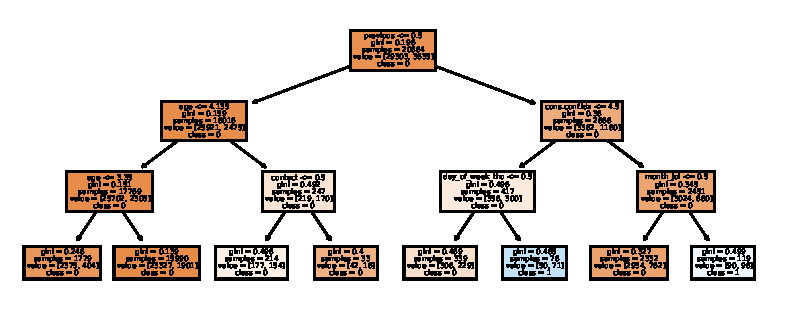
\includegraphics[width = \textwidth]{plot/classification/random_forest0.pdf}
        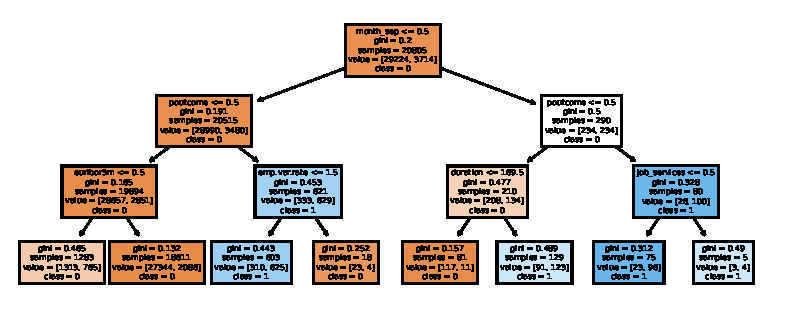
\includegraphics[width = \textwidth]{plot/classification/random_forest1.pdf}
        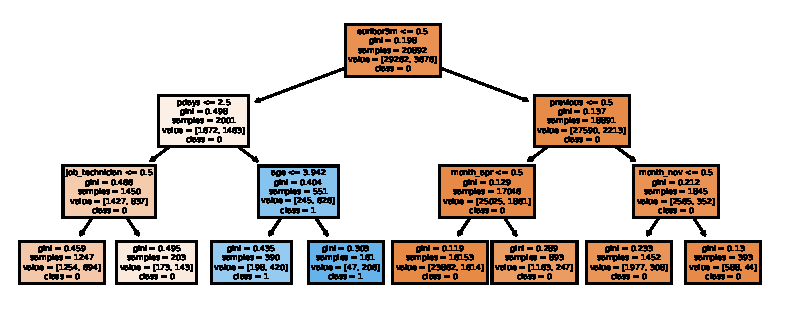
\includegraphics[width = \textwidth]{plot/classification/random_forest2.pdf}
        \caption{Random Forest}
        \label{fig:random_forest}
    \end{figure}
    
    \newpage
    \noindent
    In this simplified random forest, we obtain 10 decision trees (only 3 were printed above), then the prediction is obtained by the majority vote in the case of classification.
    
    
    \subsection{Logistic Regression} \label{logistic_regression}
    Since random forest is expansion of decision tree, we also include logistic regression to compare with former two models. Notice that plotting the logistic regression logit plot requires extremely long time for plotting ten of thousands of points, so we only use \texttt{duration} as explanatory variable to demonstrate in plot.
    \begin{figure}[!ht]
        \centering
        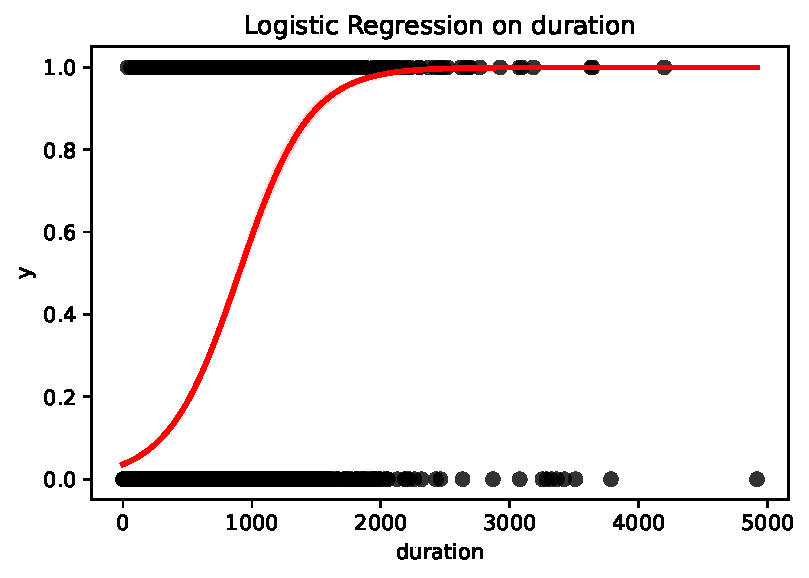
\includegraphics{plot/classification/lr/lr_duration.pdf}
        \caption{Logistic Regression on \texttt{duration}}
        \label{fig:lr}
    \end{figure}
    
    \noindent
    From the graph, we can see that using only \texttt{duration} has low accuracy, so we introduce more explanatory variables in next section.
    
    
    
    \subsection{Cross Validation and Grid Search Procedures}
    To optimize our prediction model, we use 5-fold cross validation and grid search to find the optimized parameters. This step is implemented using \texttt{Pipeline} and \texttt{GridSearchCV} from \texttt{sklearn}. The training accuracy rate, testing accuracy rate and computation time are calculated base on the best model under grid search. \\
    
    
    \begin{figure}[!ht]
        \centering
        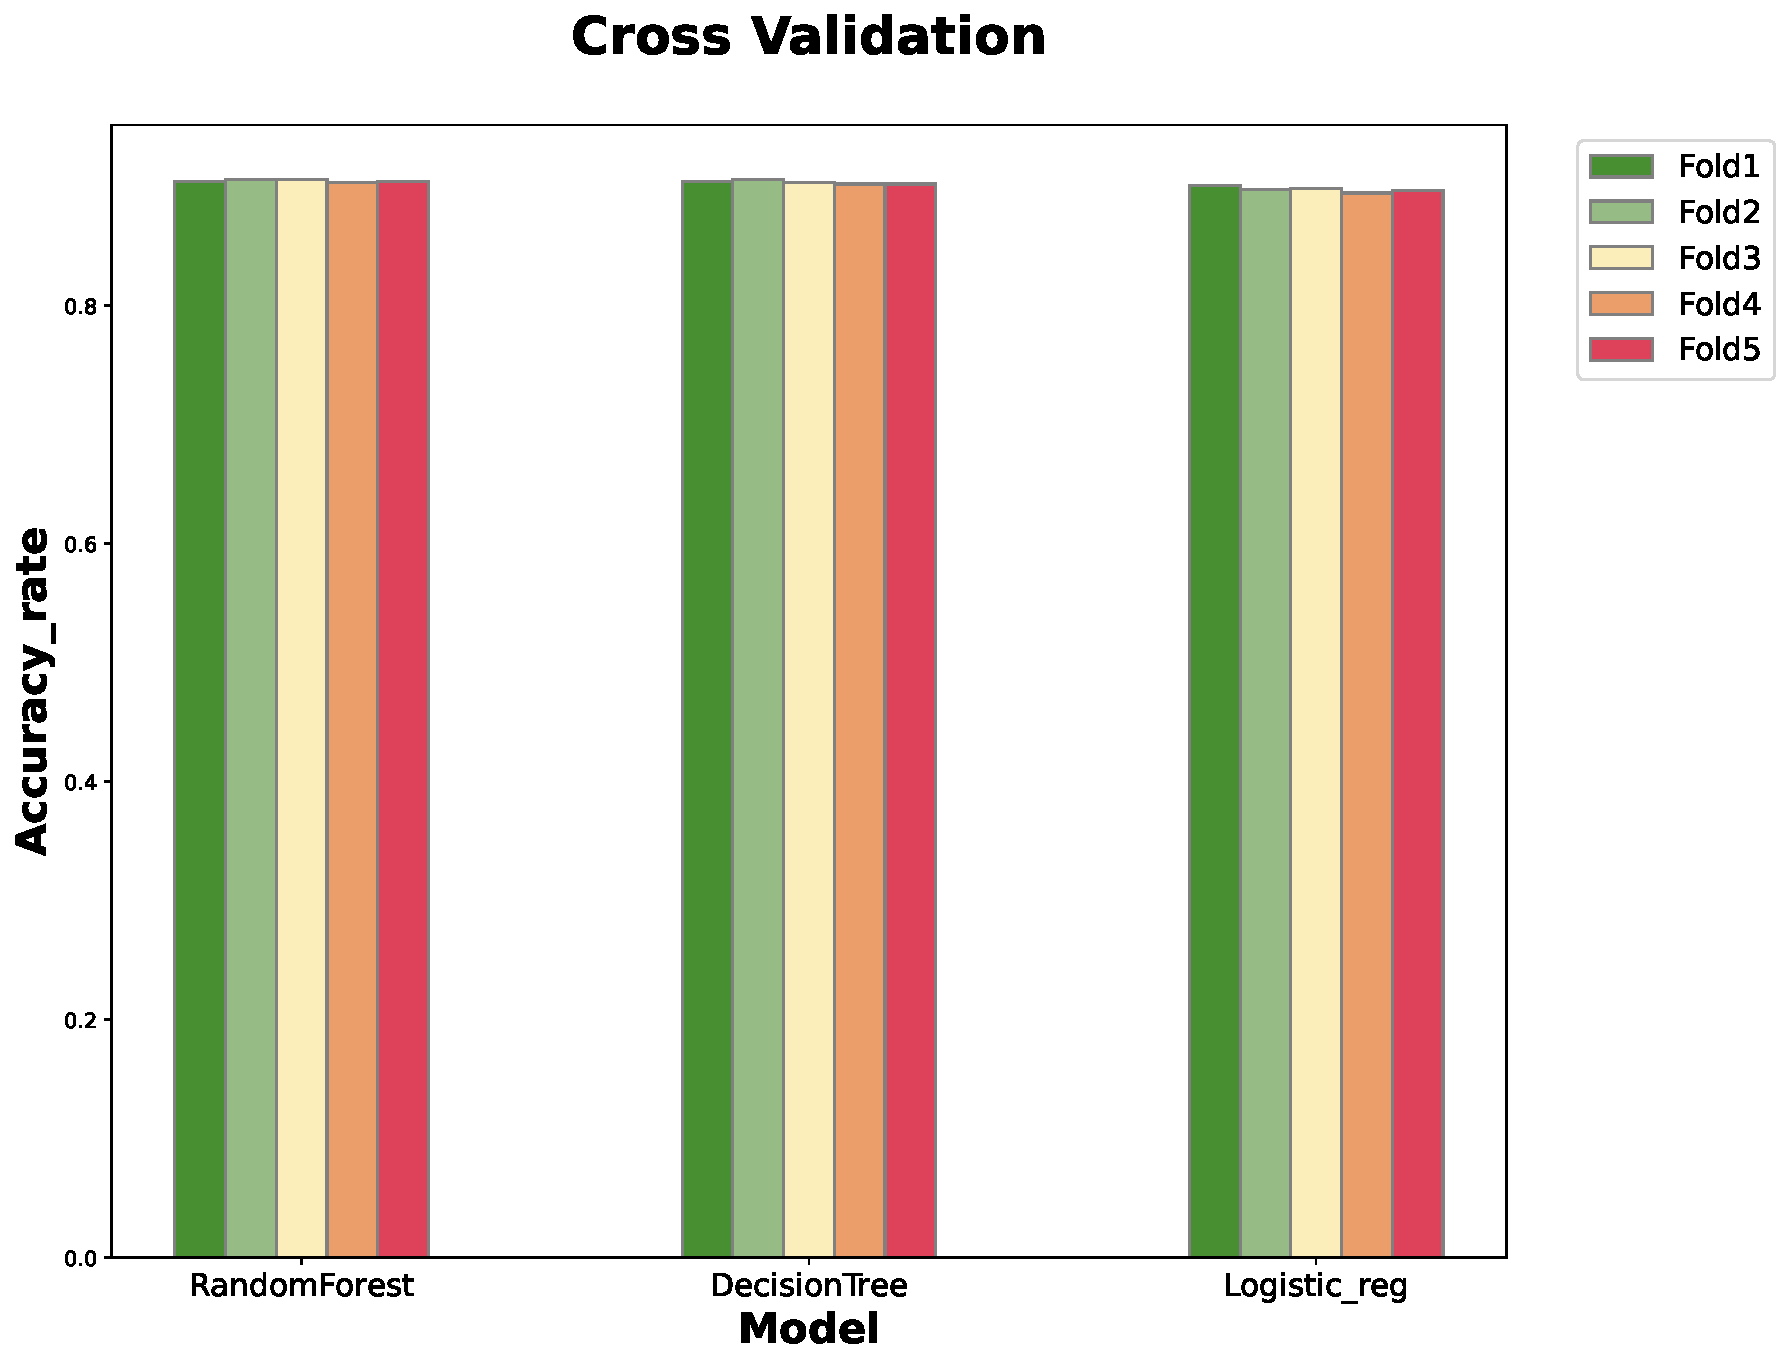
\includegraphics[width = 0.9\textwidth]{plot/classification/cv.pdf}
        \caption{Performance in Cross Validation}
        \label{fig:cv}
    \end{figure}
    
    
% \begin{lstlisting}[language = Python]
% # RandomForestClassifier
% RandomForest = Pipeline([('rf', RandomForestClassifier(n_jobs=-1,random_state=random_state))])

% # DecisionTreeClassifier
% DecisionTree = Pipeline([('dt', tree.DecisionTreeClassifier(max_features='auto',random_state=random_state))])

% # Set number of Cross Validation
% cv = StratifiedKFold(shuffle=True, n_splits=5,random_state=random_state)

% # Set parameters for RandomForestClassifier and DecisionTreeClassifier
% rf_params = [{  'rf__criterion': ['entropy'],
%                 'rf__min_samples_leaf': [80, 100],
%                 'rf__max_depth': [25, 27],
%                 'rf__min_samples_split': [3, 5],
%                 'rf__n_estimators' : [60, 70]}]

% dt_params = [{  'dt__max_depth': [8, 10],
%                 'dt__min_samples_leaf': [1, 3, 5, 7]}]

% #  Set parameters for Grid Search of RandomForestClassifier and DecisionTreeClassifier
% gs_rf = GridSearchCV(RandomForest, param_grid=rf_params,
%                      scoring='accuracy', cv=cv)

% gs_dt = GridSearchCV(DecisionTree, param_grid=dt_params,
%                      scoring='accuracy', cv=cv)

% # Models used
% model_used = [gs_rf, gs_dt]
% model_name = { 0:'RandomForest', 1:'DecisionTree'}

% # Set temp
% acc_rate = {}
% auc_rate = {}
% models = []
% time_used={}

% # Record the time used, accuracy rate and ROC rate
% for index, model in enumerate(model_used):
%         start = time.time()
%         print('Using {} model'.format(model_name[index]))
%         model.fit(x_train, y_train)
%         print('training accuracy rate is {}'.format(model.best_score_))
%         auc = roc_auc_score(y_test, model.predict_proba(x_test)[:,1])
%         print('testing accuracy rate is {} and ROC_AUC is {}'.format(model.score(x_test, y_test),auc))
%         end = time.time()
%         print('It requires {} sec to compute'.format(round(end - start, 2)))
%         print()
        
%         models.append(model.best_estimator_)
%         acc_rate[index] = model.score(x_test, y_test)
%         auc_rate[index] = auc
%         time_used[index] = round(end - start, 2)
% \end{lstlisting}
    % \noindent
    
    \newpage
    \noindent
    \textbf{Output:} (refer to source code)
    
    \noindent
    \texttt{Using RandomForest model \\
    training accuracy rate is 0.9048818398071896 \\
    ROC\_AUC: 0.9397072069254537 \\
    best parms is \{'rf\_\_criterion': 'gini', 'rf\_\_max\_depth': 25, 'rf\_\_min\_samples\_leaf': 60, \\ 'rf\_\_min\_samples\_split': 3, 'rf\_\_n\_estimators': 50\} \\
    Accuracy: 0.8990892531876138 \\
    Precision: 0.7546468401486989 \\
    Recall: 0.2097107438016529 \\
    It requires 1274.78 sec to compute \\
    \\
    Using DecisionTree model \\
    training accuracy rate is 0.9037888422385209 \\
    ROC\_AUC: 0.8968310413769026 \\
    best parms is \{'dt\_\_criterion': 'gini', 'dt\_\_max\_depth': 10, 'dt\_\_min\_samples\_leaf': 7\} \\
    Accuracy: 0.8993321190042501 \\
    Precision: 0.6026587887740029 \\
    Recall: 0.4214876033057851 \\
    It requires 3.91 sec to compute \\
    \\
    Using Logistic\_reg model \\
    training accuracy rate is 0.8977168050738198 \\
    ROC\_AUC: 0.9171117141112263 \\
    best parms is \{'lr\_\_C': 0.3, 'lr\_\_penalty': 'l1', 'lr\_\_solver': 'saga'\} \\
    Accuracy: 0.8970248937462052 \\
    Precision: 0.6578947368421053 \\
    Recall: 0.25826446280991733 \\
    It requires 244.53 sec to compute} \\
    \\
    \textbf{Confusion matrix:} \textcolor{red}{Please refer to the confusion matrix heatmap on source code.}
    

    \subsection{Comparison of Performance of Random Forest and Decision Tree}
    For reference, this running trial is performed using Intel Core$^{\text{TM}}$ i5-8250U\footnote{\url{https://ark.intel.com/content/www/us/en/ark/products/124967/intel-core-i58250u-processor-6m-cache-up-to-3-40-ghz.html}}(4C8T), 8-GB RAM.
    
    \subsubsection{Accuracy Rate, ROC rate and Computation Time}
% \begin{lstlisting}[language = Python]
% pd.DataFrame(
%     list(zip(model_name.values(), acc_rate.values(), auc_rate.values(), time_used.values())), 
%     columns = ['Model_used', 'Testing_accuracy_rate','Testing_ROC_rate','Time_used']
% )
% \end{lstlisting}
%     \noindent
    \begin{table}[ht]
        \centering
        \begin{tabular}{llrrrrr}
        {} &    Model\_used &  Accuracy &  Precision &    Recall &  ROC\_rate &  Time\_used \\
        \hline \hline
        0 &  RandomForest &  0.899089 &   0.754647 &  0.209711 &  0.939707 &    1274.78 \\
        1 &  DecisionTree &  0.899332 &   0.602659 &  0.421488 &  0.896831 &       3.91 \\
        2 &  Logistic\_reg &  0.897025 &   0.657895 &  0.258264 &  0.917112 &     244.53 \\
        \end{tabular}
        \caption{Accuracy Rate, ROC rate and Computation Time}
        \label{tab:comparison}
    \end{table}

    
    \subsubsection{ROC Graph}
% \begin{lstlisting}[language = Python]
% def plot_ROC(fpr, tpr, threshold,model):
%     trace0 = go.Scatter(x=fpr[0], y=tpr[0], text=threshold[0], fill='tozeroy', name='ROC Curve of {} '.format(model[0]))
%     trace1 = go.Scatter(x=fpr[1], y=tpr[1], text=threshold[1], fill='tozeroy', name='ROC Curve of {} '.format(model[1]))
%     trace2 = go.Scatter(x=[0,1], y=[0,1], line={'color': 'black', 'width': 1, 'dash': 'dash'}, name='Baseline')
%     data = [trace0, trace1, trace2]
    
%     layout = go.Layout(title='ROC Curve', xaxis={'title': 'False Positive Rate'}, 
%                       yaxis={'title': 'True Positive Rate'})
%     fig = go.Figure(data, layout)
%     fig.write_image("../../plot/classification/roc.pdf")
%     fig.show()

% fpr, tpr, threshold = np.transpose([
%     roc_curve(y_test, models[0].predict_proba(x_test)[:,1]), 
%     roc_curve(y_test, models[1].predict_proba(x_test)[:,1])
% ])

% plot_ROC(fpr = fpr, tpr = tpr, threshold = threshold, model = ["Random Forest", "Decision Tree"])
% \end{lstlisting}
%     \noindent
    
    \begin{figure}[H]
        \centering
        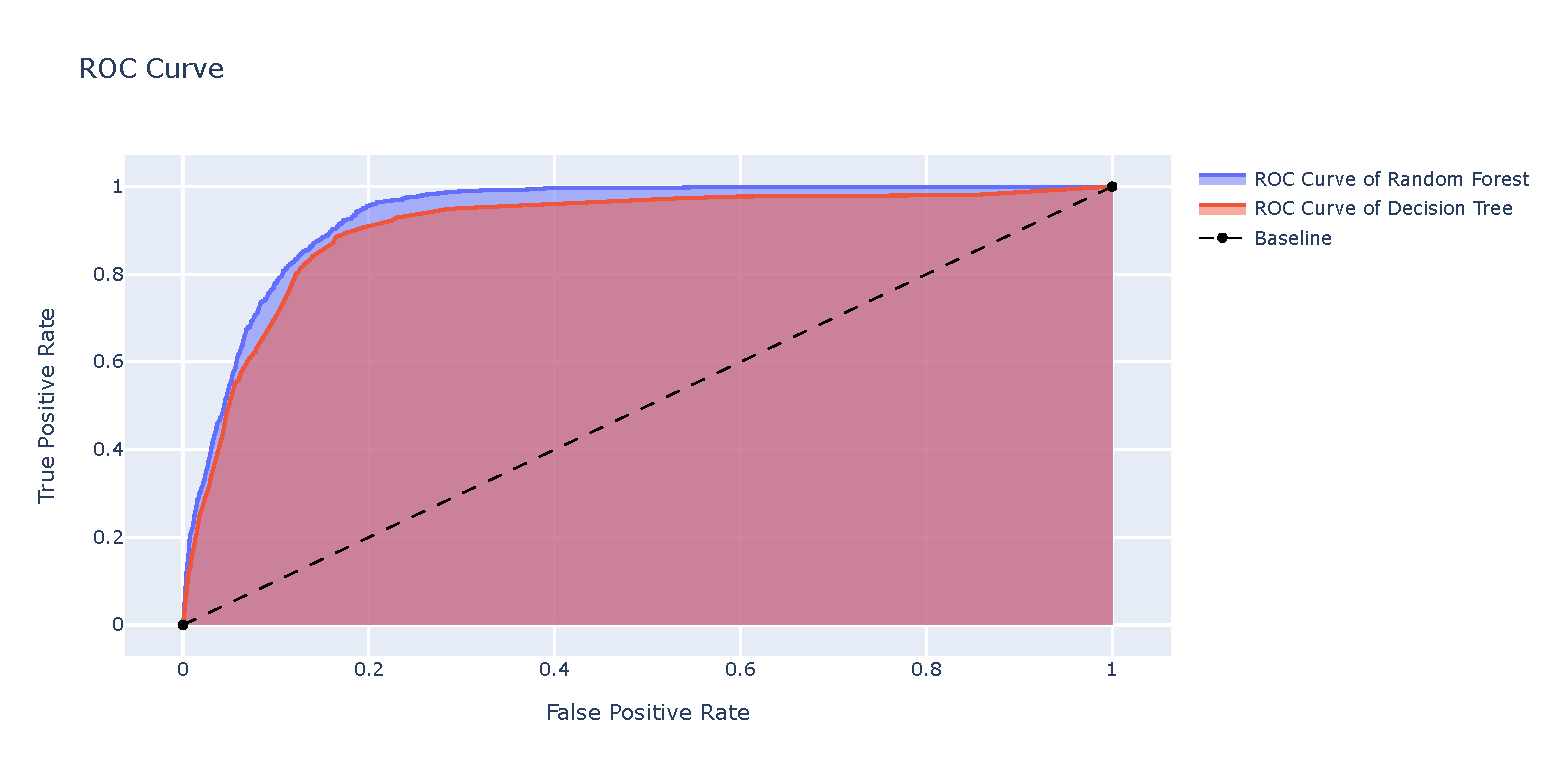
\includegraphics[width = \textwidth]{plot/classification/roc.pdf}
        \caption{ROC Graph}
        \label{fig:roc}
    \end{figure}

    
    
    \subsection{Conclusion}
    From Table \ref{tab:comparison}, random forest has the highest roc\_rate, while the accuracy rate among three models are very close. \\
    Speaking of computation time, decision tree requires shortest time, random forest requires extremely longer time relatively to others, in which decision tree only requires less than 5 seconds. \\
    From Figure \ref{fig:roc}, the roc curve of logistic regression is very close to random forest after FPR $>$ 0.3 \\
    \\
    Our group believe that random forest performs better than decision tree in this case, in terms of the accuracy in roc rate. However, in order to balance the limit of computation time, we could use logistic regression in large dataset.
    
    
    \newpage
    % \thispagestyle{empty}
    % \pagenumbering{gobble} 
    \section{Bibliography}
    \bibliographystyle{unsrt}
    % \bibliographystyle{plain} % We choose the "plain" reference style
    \bibliography{refs} % Entries are in the refs.bib file

\end{document}